\documentclass[11pt]{article}

% macros.tex — Vegas paper notation

% ── Packages ──────────────────────────────────────────────────────────
\usepackage{amsmath,amssymb,amsthm}
\usepackage{stmaryrd}
\usepackage{mathtools}
\usepackage{xcolor}
\usepackage{hyperref}
\usepackage{cleveref}
\usepackage{booktabs}
\usepackage{enumitem}
\usepackage{listings}

% ── Theorem environments ──────────────────────────────────────────────
\newtheorem{theorem}{Theorem}[section]
\newtheorem{lemma}[theorem]{Lemma}
\newtheorem{proposition}[theorem]{Proposition}
\newtheorem{corollary}[theorem]{Corollary}
\theoremstyle{definition}
\newtheorem{definition}[theorem]{Definition}
\newtheorem{example}[theorem]{Example}
\theoremstyle{remark}
\newtheorem{remark}[theorem]{Remark}

% ── Players / roles / fields ──────────────────────────────────────────
\newcommand{\Role}{\mathsf{Role}}
\newcommand{\Var}{\mathsf{Var}}
\newcommand{\Field}[2]{#1.#2}

% ── Constructs (lowercased for surface, capitalized for IR) ───────────
\newcommand{\kw}[1]{\mathbf{#1}}
\newcommand{\kjoin}{\kw{join}}
\newcommand{\kyield}{\kw{yield}}
\newcommand{\kcommit}{\kw{commit}}
\newcommand{\kreveal}{\kw{reveal}}
\newcommand{\krandom}{\kw{random}}
\newcommand{\kwithdraw}{\kw{withdraw}}
\newcommand{\kwhere}{\kw{where}}

\newcommand{\Commit}{\mathsf{Commit}}
\newcommand{\Reveal}{\mathsf{Reveal}}
\newcommand{\Public}{\mathsf{Public}}
\newcommand{\Sample}{\mathsf{Sample}}
\newcommand{\Ret}{\mathsf{Ret}}

% ── Visibility tags ───────────────────────────────────────────────────
\newcommand{\COMMIT}{\textsc{commit}}
\newcommand{\REVEAL}{\textsc{reveal}}
\newcommand{\PUBLIC}{\textsc{public}}

% ── Probability ───────────────────────────────────────────────────────
\newcommand{\PMF}[1]{\mathrm{PMF}(#1)}
\newcommand{\NN}{\mathbb{N}}
\newcommand{\RR}{\mathbb{R}}

% ── Code in prose ─────────────────────────────────────────────────────
\newcommand{\TT}[1]{\texttt{#1}}
\newcommand{\file}[1]{\texttt{#1}}

% ── Vegas listing language ────────────────────────────────────────────
\definecolor{VegasKW}{RGB}{0,80,150}
\definecolor{VegasComment}{RGB}{96,96,96}
\definecolor{VegasString}{RGB}{160,32,32}
\lstdefinelanguage{Vegas}{
  morekeywords={game,join,yield,commit,reveal,random,withdraw,macro,
                type,where,or,split,burn,null,hidden,opt,let,in,true,false,
                bool,int,address},
  sensitive=true,
  morecomment=[l]{//},
  morestring=[b]",
  keywordstyle=\color{VegasKW}\bfseries,
  commentstyle=\color{VegasComment}\itshape,
  stringstyle=\color{VegasString},
  basicstyle=\ttfamily\small,
  breaklines=true,
  showstringspaces=false,
  tabsize=2,
  columns=flexible,
}

\lstdefinestyle{vg}{
  language=Vegas,
  frame=single,
  framerule=0.4pt,
  xleftmargin=1em,
  xrightmargin=1em,
  aboveskip=0.5em,
  belowskip=0.5em,
}

\lstdefinestyle{sol}{
  language=Java, % approximate
  basicstyle=\ttfamily\small,
  frame=single,
  framerule=0.4pt,
  xleftmargin=1em,
  xrightmargin=1em,
  aboveskip=0.5em,
  belowskip=0.5em,
  morekeywords={contract,function,modifier,address,uint256,bytes32,
                bool,mapping,public,external,internal,private,view,pure,
                require,enum,return,returns,if,else,constant,immutable},
  keywordstyle=\color{VegasKW}\bfseries,
  commentstyle=\color{VegasComment}\itshape,
  stringstyle=\color{VegasString},
}


\usepackage[margin=1in]{geometry}
\usepackage{tikz}
\usetikzlibrary{arrows.meta,positioning,fit,calc,shapes.geometric,
                decorations.pathreplacing}
\usepackage[numbers,sort&compress]{natbib}

\sloppy
\emergencystretch=3em

\title{Vegas: A Domain-Specific Language for\\
       On-Chain Strategic Protocols}
\author{Elazar Gershuni\\\texttt{elazarg@gmail.com}}
\date{May 2026}

\begin{document}
\maketitle

\begin{abstract}
A smart contract that implements an auction, a voting procedure, or
any other multi-party economic mechanism is two things at once: a
program that runs on a public, adversarially ordered execution layer,
and a strategic game played by rational participants.  The contract
is usually written, audited, and deployed as the former; reasoning
about its incentive properties is left to a parallel pen-and-paper
exercise on the latter.  Vegas is a domain-specific language and
compiler that treats both views as outputs of a single specification.

A Vegas program describes a finite protocol in the natural sequential
style of a referee: who joins, who plays what, who reveals, and who
gets paid.  The compiler analyses the data flow of the specification
to build a finite \emph{event graph} --- a directed acyclic graph of
guarded writes --- and uses it as a single intermediate representation
that each backend reads in turn: (i) a Solidity (and Vyper) contract
whose execution scheduler is the dependency relation itself, with
built-in commit-reveal protection against transaction-ordering
adversaries and a timeout-driven bail-out for non-responsive
participants; (ii) a Gambit extensive-form game suitable for
equilibrium analysis; (iii) several auxiliary artifacts --- an
SMT-LIB encoding for reachability queries, a Coq/Lean witness-record
encoding of the protocol's per-step constraint structure, a
session-typed (Scribble) protocol description, and a sketch
Bitcoin/Lightning move transcript for the two-party fragment.  The expressive power of the
language is restricted by design: only finite types, no loops, no
inter-contract calls.  These restrictions are what make the whole
array of artifacts feasible to produce automatically from one source.

The report describes the language, the event-graph intermediate
representation, the automatic commit-reveal rewriting pass, the
backends, and the relationship to a companion Lean~4 library called
VegasCore.  We are explicit about the parts that are stable, the
parts that are scoped down on purpose, and the parts that we expect
to relax as the language evolves.
\end{abstract}

\tableofcontents

\section{Introduction}
\label{sec:introduction}

\subsection{Two readings, one program}

A smart contract that hosts a sealed-bid auction is one program with
two readings.  Read as an Ethereum contract, it is a state machine
exposing transactions: \TT{commit(\textit{hash})},
\TT{reveal(\textit{bid})}, \TT{settle()}.  Read as a game, it is an
extensive form with players, information sets, and a payoff
function.  These two readings are seldom kept in sync.  The
contract is written, audited, deployed, and run as a state
machine; the game is sketched, sometimes proved correct on paper,
almost never mechanically connected to the bytecode the validators
actually execute.

The gap is where strategic surprises live.  A sealed-bid auction
whose commit phase happens to publish enough information to be
front-run.  An escrow whose timeout branch creates a griefing
incentive that no equilibrium analysis predicted because the
model omitted the timeout.  A voting scheme whose Solidity
implementation reveals the tally one block earlier than the
analysis assumed.

Vegas is a small programming language and compiler aimed at this
specific gap.  A Vegas program is a finite multi-party protocol
written in the natural style of a referee: who joins, who plays
what, what is hidden and revealed when, and how the pool is split
at the end.  Programs are short --- the running examples in this
report are a dozen lines each --- and look more like the textbook
description of a game than like a smart-contract framework.  The
compiler reads the program, infers a dependency relation among
its actions, and emits a family of artifacts that all denote the
same protocol from different viewpoints: a Solidity contract for
deployment, an extensive-form game for equilibrium analysis, an
SMT-LIB encoding for reachability queries, and several others.

The premise is not that strategic correctness is proved
automatically.  The premise is that game-theoretic reasoning
about the program transfers, modulo the stated execution model,
to the deployed contract: if an analyst (or a tool) concludes that
truthful bidding is dominant in the source-language Vickrey
specification, that conclusion carries over to the Solidity
contract running on chain.  EFG generation is one channel for
that reasoning; hand analysis on the source is another;
mechanical proof in a companion Lean library is a third.  Each is
made possible by the same property: the compiler structures the
source so that the program \emph{is} a game with a public history,
information sets given by the visibility discipline, and a
payoff function over the terminal state, and every backend is a
lowering of that game.

This report describes how that compilation is organized, what
the language can and cannot express, how the central
intermediate representation --- the \emph{event graph} ---
captures the strategic structure of a protocol, and how the
per-backend lowerings are constrained so that the artifacts agree.

\subsection{What Vegas is and is not}

Vegas is deliberately narrow.  The aim is to make the round trip from
specification to deployed contract to game-theoretic analysis short
and reliable for a useful class of protocols, not to be a general
purpose smart-contract language.  Concretely, in scope are:

\begin{itemize}\itemsep1pt
\item finite, terminating multi-party protocols with a single
  pool of locked funds;
\item bounded types (booleans, finite ranges, enumerations);
\item deterministic guards (\TT{where} clauses) over prior public
  values and over the value being written;
\item public randomness via an explicit \texttt{random} construct;
\item commit-reveal patterns, with automatic insertion when the
  compiler detects simultaneous public moves that would otherwise be
  front-runnable;
\item explicit operational handling of non-responsive participants
  (timeouts and bail-outs, with handler clauses chosen by the
  programmer);
\item terminal allocation of the pool by a \TT{withdraw} clause.
\end{itemize}

Out of scope, on purpose:

\begin{itemize}\itemsep1pt
\item unbounded data and loops --- the event graph must be finite;
\item ERC-20/ERC-777 token flows and multi-token games (planned, not
  in the current language);
\item interactions with arbitrary other contracts (the protocol is a
  closed system; cross-contract MEV is parameter, not modelled);
\item private randomness from outside oracles;
\item dynamic player counts (the role set is fixed at compile time).
\end{itemize}

These restrictions are real costs.  They are also what make the
multi-backend story feasible: every artifact is computed by
exhaustive enumeration or simple recursion over a finite graph, with
no need to approximate or to choose a sound-but-incomplete encoding.
A Gambit extensive-form game can be built directly from the
EventGraph because the graph is finite; an SMT-LIB encoding of
``can role $R$ reach a configuration where they get $\geq x$ wei?''
is quantifier-free over a finite set of action witnesses; a Lean or
Coq witness-record encoding terminates by construction.  We expect
the language to grow --- variable deposits, tokens, bounded
iteration --- and we have tried to make the IR robust enough to
accommodate those extensions.  The current paper documents the
foundations.

\subsection{A first example}
\label{sec:intro:first-example}

The following Vegas program is the complete specification of a
distribution-semantics Monty Hall game.  Two roles, Host and Guest,
each lock 20 wei of deposit into a 40 wei pool.  The Host hides the
car behind one of three doors; the Guest picks a door; the Host
reveals a goat door; the Guest decides whether to switch; the Host
reveals the car; payouts are computed from the public transcript.
If a role fails to act in time, the \texttt{or split} handler
forfeits their deposit to the surviving party.

\begin{lstlisting}[style=vg]
type door = {0, 1, 2}

game main() {
  join Host()  $ 20;
  join Guest() $ 20;
  commit or split Host(car: door);
  yield  or split Guest(d: door);
  yield  or split Host(goat: door) where Host.goat != Guest.d;
  yield  or split Guest(switch: bool);
  reveal Host(car: door) where Host.goat != Host.car;
  withdraw { Guest -> ((Guest.d != Host.car) <-> Guest.switch) ? 40 : 0;
             Host  -> ((Guest.d != Host.car) <-> Guest.switch) ? 0  : 40 }
}
\end{lstlisting}

From this twelve-line source Vegas produces every artifact listed
in the abstract: a roughly two-hundred-line Solidity contract that
enforces the protocol step by step (with cryptographic commitments
for the Host's hidden door and a fall-back to the \TT{or split}
clauses when a role times out); an extensive-form game in
Gambit's format, containing the move tree and the information
sets induced by the dependency relation; an SMT-LIB
witness-existence encoding; and a Coq/Lean witness-record
encoding (the Diamond DAG of \S\ref{sec:other:diamond}).  All are
produced by the current compiler and exercised by the
golden-master test suite.  The Solidity output is deployable to a
local Anvil node; fed to Gambit, the EFG returns the
``always switch'' equilibrium for Monty Hall.  Nothing in the
twelve-line source mentions Ethereum, cryptographic commitments,
timeouts, gas, or game trees.

The example is small enough to verify by inspection that the two
artifacts agree on what they say is hidden, what is public, when
each player observes what, and which deviations are punished.  At
larger scale the agreement has to be argued, not inspected --- which
is what motivates the companion Lean formalization VegasCore
discussed in \S\ref{sec:vegascore}.

\subsection{Why an event graph}
\label{sec:intro:why-graph}

A natural alternative would be to compile the surface syntax
directly to a state machine for Solidity and directly to a tree
for Gambit, twice, with the two backends owning their own
semantics.  That is also what an experienced human writes by hand
when they want both views of the same protocol.  Vegas does not
do this for three reasons.

First, the textual order of the Vegas source does \emph{not} encode
the strategic structure.  In the Monty Hall example above, the line
\TT{yield Guest(d: door)} appears below the Host's hidden
\TT{commit}.  But the Guest cannot read the Host's hidden value, and
the Host's commit has no data dependency on the Guest; the two
actions are concurrent in the strategic sense, regardless of the
order they happen to be typed in.  Compiling to a tree directly
would force an arbitrary ordering choice, which then has to be
``undone'' with information-set equivalences.  Inferring
concurrency from data dependencies once, in the IR, and letting
every backend read it off the same graph, is simpler.

Second, the operational behaviour of a Solidity contract is more
naturally described by a dependency relation than by a global step
counter.  The Solidity backend emits a \TT{depends} modifier per
action, the modifier gating execution on the completion flags of
the action's predecessors in the event graph; concurrent actions
can arrive in any order.  This matches the on-chain reality (the
transaction ordering is chosen by builders, not by the contract)
without the contract having to encode a totalisation.

Third, the rewriting passes the compiler performs --- in particular,
automatic commit-reveal insertion --- are dependency-graph rewrites.
They are easier to state and easier to test on a graph than on the
syntax tree.

So Vegas uses a single intermediate representation, the
\emph{EventGraph}, between the surface language and every backend.
Each backend reads the graph; no backend reaches behind the graph
to the surface syntax.  Section~\ref{sec:eventgraph} defines the
EventGraph in detail; the rest of the report uses it pervasively.

\subsection{Contributions and outline}
\label{sec:intro:contributions}

The contributions of this report are:

\begin{enumerate}\itemsep2pt
\item \emph{A language design} (\S\ref{sec:language}) that makes it
  feasible to describe a finite on-chain protocol in fewer than
  twenty lines and that compiles, without further specification,
  to both deployable code and a game-theoretic model.

\item \emph{The EventGraph IR} (\S\ref{sec:eventgraph}) and its
  associated invariants (acyclicity, commit-reveal ordering,
  visibility on guard reads), capturing concurrency, observability,
  and the protocol's information-set structure in one finite
  object.

\item \emph{Automatic commit-reveal insertion}
  (\S\ref{sec:commit-reveal}): a graph-rewriting pass that detects
  concurrent public writes and replaces each one with a
  commit-then-reveal pair, with predecessors set up so that no
  player can observe another player's reveal before committing
  themselves.  This addresses one specific subclass of MEV ---
  observation-before-action on simultaneous moves within the
  protocol --- by making the mitigation a structural property
  of the IR rather than an implementation discipline.

\item \emph{A family of backends} (\S\S\ref{sec:solidity}--\ref{sec:other-backends})
  that each consume the same EventGraph: Solidity and Vyper for
  EVM deployment with \TT{depends}-modifier scheduling and a
  timeout-driven bail-out for non-responsive participants; Gambit
  for extensive-form game generation via frontier exploration;
  SMT-LIB for reachability queries; Scribble for the session-typed
  protocol description; a sketch Bitcoin/Lightning move transcript
  for the two-party fragment (a textual artifact, not deployable
  bytecode); a Coq/Lean ``Diamond DAG'' witness-record encoding
  that captures the per-step constraint bundle as a dependent
  type.

\item \emph{An operational handler layer}
  (\S\ref{sec:liveness}) for liveness and griefing: every action
  can be guarded by a handler that fires if the actor does not
  respond within a deadline.  The handler is a strategic choice
  available to the actor (``quit''), realised by the Solidity
  backend through a timeout-and-bail mechanism, and exposed to the
  game-theoretic backends as an explicit move.

\item \emph{A bridge to a Lean~4 formalization}
  (\S\ref{sec:vegascore}) named VegasCore, which formalizes a core
  calculus over the same EventGraph carrier.  Vegas and VegasCore
  are independent artifacts: Vegas is a compiler tool, VegasCore is
  a self-contained semantic construction.  Where they describe the
  same object they use the same name; where they diverge, the
  divergence is recorded.

\item \emph{An example library} (\S\ref{sec:evaluation}):
  thirty-nine Vegas specifications covering classical mechanisms
  (Vickrey auction, Prisoners' Dilemma, Centipede), Ethereum
  patterns (escrow, micropayment channel, governance voting), and
  adversarial constructions (front-running setups, hidden-reserve
  auctions).  Each example is compiled to every applicable
  backend.
\end{enumerate}

The report follows the order of the compiler.
\S\ref{sec:language} introduces the surface language and walks
through one example end-to-end.  \S\ref{sec:eventgraph} fixes the
pipeline and defines the EventGraph and its invariants.  \S\ref{sec:commit-reveal} describes the
automatic commit-reveal pass.  \S\S\ref{sec:solidity}--\ref{sec:other-backends}
cover the backends.  \S\ref{sec:liveness} describes the
liveness/quit-handler layer.  \S\ref{sec:vegascore} maps the
construction onto the companion Lean formalization.
\S\ref{sec:evaluation} reports on the example suite.
\S\S\ref{sec:related}--\ref{sec:discussion} close with related work
and a frank discussion of current limitations and natural
extensions.

\section{The Vegas Language}
\label{sec:language}

This section introduces the surface language by example, fixes
intuitive semantics for each construct, and gives the small grammar
in BNF.  The next section traces what happens to a program once the
compiler takes it apart.

\subsection{Programs and roles}

A Vegas program declares optional type aliases and macros, then a
single top-level \TT{game} block.  The block names the roles, opens a
\TT{join} phase that locks each role's deposit into a common pool,
and proceeds with a sequence of action statements until a
\TT{withdraw} clause splits the pool.

\begin{lstlisting}[style=vg]
type bid = {0 .. 10}

game main() {
  join Seller() $ 0
       Bidder() $ 100;
  // ... statements ...
  withdraw { Seller -> ...; Bidder -> ... }
}
\end{lstlisting}

Role identifiers start with an uppercase letter; field names with
lowercase.  A field is always identified relative to its owning
role: \TT{Bidder.b} denotes the field \TT{b} of role \TT{Bidder}.
Each field has at most one writing action; the language has no
explicit reassignment.

\subsection{Action statements}

There are five action kinds.  Three of them (\TT{yield},
\TT{commit}, \TT{reveal}) write one or more fields owned by
the actor; \TT{join} and \TT{random} declare a role
(strategic and chance, respectively) and record its deposit,
without writing protocol fields.

\paragraph{\TT{join}.}  Initial deposit and admission.  The
\TT{join} phase appears once, at the top of the game.  A role listed in the join phase is bound to the game, with its
deposit locked into the pool.

\paragraph{\TT{yield}.}  A public move.  The actor declares a value
of a given type:
\begin{lstlisting}[style=vg]
yield Guest(d: door);
\end{lstlisting}
After this action fires, \TT{Guest.d} is visible to every role.  A
\TT{yield} can carry a \TT{where} guard, e.g.
\TT{yield Host(goat: door) where Host.goat != Guest.d}; this guard
is enforced when the move is played.

\paragraph{\TT{commit}.}  A private move.  The actor declares a
value that is held cryptographically (in the deployed contract:
under a hash with salt) until a later \TT{reveal}:
\begin{lstlisting}[style=vg]
commit Host(car: door);
// ...
reveal Host(car: door) where Host.goat != Host.car;
\end{lstlisting}
A \TT{where} clause on a \TT{commit} is \emph{deferred}: it is
checked at the matching \TT{reveal}, not at the commit, because the
committed value is not yet observable.

\paragraph{\TT{reveal}.}  Make a previously committed field
public.  Every \TT{commit} is paired with exactly one \TT{reveal}
on each non-quit path through the game; the type checker enforces
this (a committed value that is never revealed and never reachable
through a quit handler is rejected).  Before reveal, only the
committing actor knows the value --- operationally, the contract
holds only the hash.

\paragraph{Randomness.}  Vegas distinguishes two surface forms,
matching the two operational modes available on EVM today.

A \TT{random} declaration introduces a chance role with an actor
identity but no deposit: useful when the draw is \emph{private}
and must be committed and later revealed by a designated actor.
\begin{lstlisting}[style=vg]
random Host;
commit Host(car: door ~ uniform { 0, 1, 2 });
reveal Host(car: door);
\end{lstlisting}
A \TT{sample} declaration introduces an \emph{anonymous public}
draw with no actor:
\begin{lstlisting}[style=vg]
sample (w: ticket);
\end{lstlisting}
Anonymous samples live under a reserved label \TT{Sample}; their
value is computed on chain from \TT{block.prevrandao} with
domain separation.  No actor identity is required; the field is
referenced in expressions as \TT{Sample.w}.

A parameter may carry a \emph{distribution annotation}
\TT{$\sim$ \textit{D}} declaring its analysis prior.  Two surface
forms are available, both finite-support and rational-weighted:
\TT{uniform \{ \dots \}} and
\TT{weighted \{ v\textsubscript{1}: w\textsubscript{1}, \dots \}}.
The annotation is an \emph{analysis assumption}: the analysis
backends (Gambit, MAID) interpret the action as a draw from the
declared distribution.  On a strategic role's action it asserts
that the role plays through; on a chance role's or sample's
action it overrides the default uniform-over-domain prior.

\paragraph{Trust model for random sources.}
Random sources are trusted to follow the declared (or assumed
uniform) distribution.  There is no penalisation, no quit, no
slash; if a \TT{random} actor commits an out-of-support value and
refuses to reveal, the game stalls with funds held in the
contract.  A guard on a chance node is interpreted as standard
probabilistic conditioning, \TT{$\sim D$ where $\varphi$} meaning
``the value is drawn from the conditional distribution $D \mid
\varphi$''.  The MAID emitter projects self-only guards
statically into a renormalised CPD; the Gambit emitter
conditions per trace; both reject \TT{where false}.

\paragraph{Independent public moves.}  Multiple roles can appear in a
single statement.  Strategically, these are simultaneous moves:
no role is allowed to condition its choice on another role's
choice from the same statement.
\begin{lstlisting}[style=vg]
yield or split A(c: bool) B(c: bool);
\end{lstlisting}
This is exactly the situation that would invite front-running if
written naively, and is the canonical input to the automatic
commit-reveal pass described in \S\ref{sec:commit-reveal}.

\subsection{Guards and views}
\label{sec:lang:guards}

A guard is a \TT{where} clause attached to an action.  Its scope is
the snapshot of fields visible \emph{just before} the action fires,
plus the field being written.  Two distinctions matter.

\emph{Self-only versus contextual guards.}  A guard that references
only the field being written (\TT{where x != 2}) constrains the
domain of that field; a guard that references prior fields
(\TT{where Host.goat != Guest.d}) constrains the legality of a move
based on the public history.  Both are allowed.  Both are
statically required to reference only fields the actor can observe
at this point.

\emph{Public versus private fields.}  An actor cannot observe
another actor's hidden field; therefore a guard cannot read it.
The compiler rejects programs that try (it cannot enforce a
constraint nobody can check).  When the guard is on a
\TT{commit}, however, the actor's own freshly written field is
private to them: the constraint is recorded and re-checked when
the value is revealed, so that any later observer can verify the
constraint at reveal time.

\subsection{Quit handlers}

Real protocols have to cope with a player who stops responding.
Vegas treats this as a strategic move named \TT{Quit}: at any point
where a role is expected to act, the role can choose to abandon the
game.  What happens next is specified by an \emph{or-handler} on
the action:
\begin{lstlisting}[style=vg]
yield or split Guest(d: door);
yield or burn  A(c: bool);
yield or null  Odd(c: bool) Even(c: bool);
\end{lstlisting}
The handlers do the following:
\begin{itemize}\itemsep1pt
\item \TT{split} --- the quitter's deposit is split among the
  surviving roles.  In a two-player game, this is forfeit.
\item \TT{burn} --- the quitter's deposit is destroyed (or sent to
  a designated burn address).
\item \TT{null} --- the missing value becomes \TT{null} (typed
  \TT{opt T}); downstream actions and the \TT{withdraw} clause are
  required to handle the optional case.
\end{itemize}
Operationally the handler fires when a timeout elapses without the
expected action.  At the game-theoretic level, \TT{Quit} is just
another move available to the actor; equilibrium analyses see it
explicitly.  \S\ref{sec:liveness} treats the subgame structure in
detail.

\subsection{Withdraw and conservation}

A game terminates by reaching a \TT{withdraw} clause, which
allocates the entire locked pool.  Outcomes are
brace-delimited blocks of \TT{role -> exp} entries; an outcome
may additionally carry a single \TT{burn N} item that records
how much of the pool is destroyed (or, in the EVM emission,
retained in the contract permanently).  \TT{withdraw} can be
conditional:
\begin{lstlisting}[style=vg]
withdraw (A.c && B.c) ? { A -> 100; B -> 100 }
       : (A.c)        ? { A -> 200; B -> 0   }
       : (B.c)        ? { A -> 0;   B -> 200 }
       :                { A -> 90;  B -> 110 }
\end{lstlisting}
Conservation --- that, on every reachable terminal branch, the
sum of role payouts and the burn equals the sum of strategic
deposits --- is enforced statically.  The compiler runs the same
extensive-form enumeration the Gambit backend uses, and at each
terminal checks the per-branch equation; any underpayment (funds
stuck) or overpayment (contract reverts) is reported as a static
error.  Chance roles and anonymous samples have no claim on the
pool and so do not appear in withdraw payouts: their share, if
any, is recorded as a \TT{burn}.

\subsection{Types}

Vegas types are deliberately small.  The base types are:

\begin{itemize}\itemsep1pt
\item \TT{bool};
\item finite enumerations (\TT{type door = \{0, 1, 2\}}) and
  finite ranges (\TT{type bid = \{0..10\}});
\item \TT{address} (used only in joins and metadata; not first-class
  in payoff expressions);
\item \TT{int} (mapped to a 256-bit integer in the EVM backends; the
  Gambit backend rejects unbounded \TT{int} in moves because it
  needs a finite move alphabet).
\end{itemize}

Two type modifiers --- \TT{hidden} and \TT{opt} --- are
introduced by the compiler rather than written in source.  A
\TT{commit} action's parameter is implicitly typed
\TT{hidden T}: the value is private to the committing actor
until the matching \TT{reveal} fires.  A field associated with
an \TT{or null} handler is implicitly typed \TT{opt T}, marking
that it may be \TT{null} when the actor takes the \TT{Quit}
branch; the language requires \TT{withdraw} expressions to
handle the \TT{null} case explicitly.

\subsection{Macros}

Macros are hygienic expression-level abbreviations, inlined before
the IR is built.  They simplify reasoning about non-trivial
mechanisms; Vickrey auctions, for instance, are easier to read
with a \TT{secondMax} macro.

\begin{lstlisting}[style=vg]
macro max2(a: bid, b: bid): bid = (a >= b ? a : b);
macro secondMax(a: bid, b: bid, c: bid): bid =
    (a == max3(a,b,c)) ? max2(b, c)
  : (b == max3(a,b,c)) ? max2(a, c)
  :                      max2(a, b);
\end{lstlisting}

Macros expand syntactically; recursion is disallowed.  Macro
expansion is purely textual at the expression level: macros do
not introduce new actions or rewrite the action sequence.

\subsection{A walked example: Vickrey auction}
\label{sec:lang:vickrey}

Putting the constructs together, here is a three-bidder sealed-bid
second-price (Vickrey) auction with a fixed-domain bid type.  The
\TT{yield or split} statement carries three actor heads, declaring
the three bids as independent public choices.

\begin{lstlisting}[style=vg]
type bid = {0 .. 2}

macro max2(a: bid, b: bid): bid = (a >= b ? a : b);
macro max3(a: bid, b: bid, c: bid): bid = max2(max2(a, b), c);
macro secondMax(a: bid, b: bid, c: bid): bid =
    (a == max3(a,b,c)) ? max2(b, c)
  : (b == max3(a,b,c)) ? max2(a, c)
  :                      max2(a, b);
macro isWinner(myBid: bid, b1: bid, b2: bid, b3: bid): bool =
    (myBid == max3(b1, b2, b3));

game main() {
  join Seller() $ 100 B1() $ 100 B2() $ 100 B3() $ 100;

  yield or split
    B1(b: bid)
    B2(b: bid)
    B3(b: bid);

  withdraw {
    Seller -> 100 + secondMax(B1.b, B2.b, B3.b);
    B1 -> isWinner(B1.b, B1.b, B2.b, B3.b)
            ? (100 - secondMax(B1.b, B2.b, B3.b)) : 100;
    B2 -> isWinner(B2.b, B1.b, B2.b, B3.b)
            ? (100 - secondMax(B1.b, B2.b, B3.b)) : 100;
    B3 -> isWinner(B3.b, B1.b, B2.b, B3.b)
            ? (100 - secondMax(B1.b, B2.b, B3.b)) : 100;
  }
}
\end{lstlisting}

The compiler does not assume the front-running problem has been
solved.  It reads three independent public moves and rewrites the
EventGraph so that each bidder commits to a hash first and reveals
later, with every reveal gated on every other bidder's commit.
The resulting Solidity contract implements a sealed-bid auction;
the resulting Gambit game has each bidder choose a hidden value in
a common information set.  Both come from the same source.

\subsection{Grammar}

For reference, the full surface grammar lives in the ANTLR file
\file{Vegas.g4} at the project root; the salient productions are
roughly:
\begin{align*}
\mathit{program} &::= (\mathit{typeDec} \mid \mathit{macroDec})^*\ \TT{game}\ \mathit{ident}\ \TT{()}\ \TT{\{}\ \mathit{ext}\ \TT{\}}\\
\mathit{ext} &::= \mathit{kind}\ (\texttt{or}\ \mathit{handler})?\ \mathit{query}^+\ \TT{;}\ \mathit{ext}\\
             &\mid \TT{random}\ \mathit{role}\ (\TT{()})?\ \TT{;}\ \mathit{ext}\\
             &\mid \TT{sample}\ \TT{(}\ \mathit{varDec}^+\ \TT{)}\ \TT{;}\ \mathit{ext}\\
             &\mid \kwithdraw\ \mathit{outcome}\\
\mathit{kind} &::= \kjoin \mid \kyield \mid \kreveal \mid \kcommit\\
\mathit{query} &::= \mathit{role}\ \TT{(}\ \mathit{paramDec}^*\ \TT{)}\ (\$\,\mathit{int})?\ (\kwhere\ \mathit{exp})?\ (\TT{||}\ \mathit{queryHandler})?\\
\mathit{paramDec} &::= \mathit{name}\ \TT{:}\ \mathit{type}\ (\TT{$\sim$}\ \mathit{dist})?\\
\mathit{dist} &::= \TT{uniform \{ \dots \}} \mid \TT{weighted \{ }\mathit{v}\TT{:}\,\mathit{w},\dots\ \TT{\}}\\
\mathit{handler} &::= \TT{split} \mid \TT{burn} \mid \TT{null}\\
\mathit{item} &::= \mathit{role}\ \TT{->}\ \mathit{exp} \mid \TT{burn}\ \mathit{exp}
\end{align*}
The \TT{random} production does not admit \TT{\$ deposit}: chance
actors do not stake.  The grammar is unsurprising; what makes
Vegas work is the analysis done in the next several sections.

\section{The EventGraph}
\label{sec:eventgraph}

This section introduces the EventGraph: the finite,
visibility-aware directed acyclic graph that all Vegas backends
read.  The graph is the structural core of the language; every
backend-facing notion --- front-running mitigation, information-set
construction, bail-out handling --- is expressed as a property of
this graph or as a rewrite on it.  The frontend pipeline below
treats it as the only stable interface between source and
artifacts.

\begin{center}
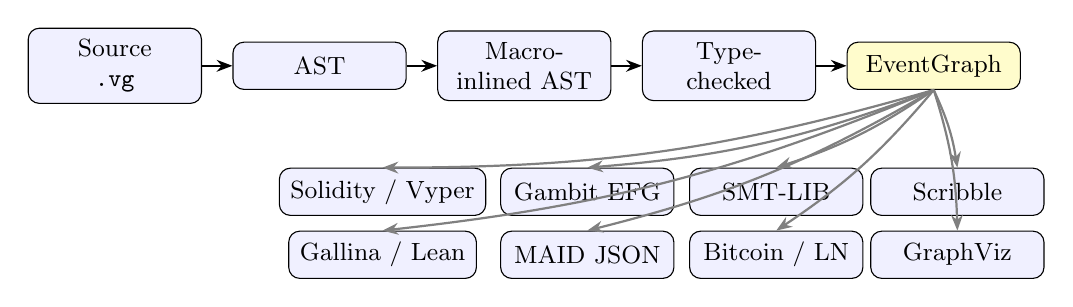
\begin{tikzpicture}[
  every node/.style={font=\small},
  box/.style={draw, rounded corners, inner sep=4pt, minimum width=2.2cm,
              minimum height=6mm, fill=blue!6, align=center},
  ir/.style ={draw, rounded corners, inner sep=4pt, minimum width=2.2cm,
              minimum height=6mm, fill=yellow!20, align=center},
  arr/.style={-{Stealth[length=2mm]}, thick}
]
\node[box] (src) at (0,0) {Source\\\TT{.vg}};
\node[box] (ast) at (2.6,0) {AST};
\node[box] (mac) at (5.2,0) {Macro-\\inlined AST};
\node[box] (chk) at (7.8,0) {Type-\\checked};
\node[ir]  (eg)  at (10.4,0) {EventGraph};

\node[box] (sol) at (3.4,-1.6) {Solidity / Vyper};
\node[box] (gam) at (6.0,-1.6) {Gambit EFG};
\node[box] (smt) at (8.4,-1.6) {SMT-LIB};
\node[box] (scr) at (10.7,-1.6) {Scribble};
\node[box] (gal) at (3.4,-2.4) {Gallina / Lean};
\node[box] (mai) at (6.0,-2.4) {MAID JSON};
\node[box] (btc) at (8.4,-2.4) {Bitcoin / LN};
\node[box] (gv)  at (10.7,-2.4) {GraphViz};

\draw[arr] (src) -- (ast);
\draw[arr] (ast) -- (mac);
\draw[arr] (mac) -- (chk);
\draw[arr] (chk) -- (eg);

\foreach \t in {sol, gam, smt, scr, gal, mai, btc, gv}
  \draw[arr, gray] (eg.south) to[bend left=8] (\t.north);
\end{tikzpicture}
\end{center}

The frontend (\file{vegas/frontend/}) parses with an
ANTLR-generated parser, inlines macros, and runs a four-pass type
checker that validates type aliases, macro signatures, the
protocol's join/yield/reveal/commit/withdraw structure, and the
visibility discipline of guards.  It then lowers to an
intermediate representation \TT{GameIR}, which packages the
EventGraph together with a per-role payoff expression and the
chance-role set.  Two transformation passes operate on the IR: the
first builds the EventGraph from typechecked AST (described in
this section), the second is the commit-reveal expansion pass
(\S\ref{sec:commit-reveal}) that rewrites concurrent public writes
into commit-then-reveal pairs.  Backends consume the post-rewrite
graph.

\subsection{Nodes}

A node of the EventGraph represents one statement in the protocol:
a \TT{join}, a \TT{yield}, a \TT{commit}, a \TT{reveal}, or a
\TT{random}.  Each node is identified by a pair
$\mathit{NodeId} = (\Role, n)$ where $\Role$ is the actor and $n$
is an integer giving the node's source position.  The pair is
stable: it is fixed at IR construction time and used throughout
backends as a deterministic identifier.

To each node the IR attaches a payload of three pieces:

\begin{itemize}\itemsep1pt
\item the \emph{specification} (\TT{NodeSpec}): the parameter list,
  any deposit (for \TT{join} nodes), and the guard expression;
\item the \emph{structural metadata} (\TT{NodeStruct}): the owner,
  the set of written fields, the visibility of each written field
  (one of \COMMIT, \REVEAL, \PUBLIC), and the set of fields the
  guard reads from prior nodes;
\item a derived \emph{kind} (\TT{Visibility}), which is the
  ``dominant'' visibility of the node's writes ---
  \COMMIT for hidden writes, \REVEAL for matching reveals,
  \PUBLIC for plain writes.
\end{itemize}

The split between \TT{NodeSpec} and \TT{NodeStruct} is mainly an
engineering choice: backends that need only structural information
(the Gambit and Scribble backends, primarily) can ignore the spec.

\subsection{Edges and dependency inference}
\label{sec:eventgraph:edges}

Edges in the EventGraph represent control or data dependencies.
The IR builds them by analysing the typechecked AST.  An edge
$A \to B$ means $B$ cannot fire until $A$ has fired.  The
compiler installs an edge $A \to B$ when any of the following
holds:

\begin{itemize}\itemsep1pt
\item \emph{Phase order.}  If $A$ and $B$ are in adjacent source
  phases (consecutive top-level statements), $A \to B$.  This
  preserves the textual ordering at the granularity of phases,
  which is what the programmer can rely on.
\item \emph{Guard read.}  If $B$'s guard reads a field $f$, and
  the latest writer of $f$ before $B$ is $A$, then $A \to B$.
  The guard cannot evaluate until the value is available.
\item \emph{Commit before reveal.}  If $B$ is a \REVEAL of field
  $f$ and $A$ is the \COMMIT of $f$, then $A \to B$.  The reveal
  must come after its commit.
\end{itemize}

Within a single phase, multiple roles can act simultaneously (they
appear in the same \TT{yield}/\TT{commit} statement).  Their nodes
share predecessors and are not connected to each other: they are
concurrent in the dependency graph, which is what justifies
treating them as simultaneous moves in the strategic analysis.

\subsection{Visibility}
\label{sec:eventgraph:visibility}

Each written field has a visibility tag that records what an
observer learns from the corresponding write.  The three tags are:

\begin{description}\itemsep1pt
\item[\PUBLIC.]  The value is public from the moment of the write.
  Any later node may read it.
\item[\COMMIT.]  The value is hidden.  Operationally, only its
  cryptographic commitment is public; the actor knows the value;
  no other actor learns it from this node.
\item[\REVEAL.]  A previously committed value is now public.  The
  reveal is paired with the unique prior commit of the same field.
\end{description}

The IR ensures that visibility is consistent with the dependency
relation.  In particular:

\begin{itemize}\itemsep1pt
\item every \REVEAL is reachable from its matching \COMMIT;
\item every field referenced by a guard at node $B$ has either
  been written \PUBLIC by some predecessor of $B$, or has been
  revealed by some predecessor of $B$ (so its value is known
  publicly at $B$);
\item the owner of a node always sees their own writes (an actor
  may guard their action on a field they have just decided ---
  this is how self-only guards like \TT{where x != 2} are
  modelled).
\end{itemize}

If any of these conditions fails, the EventGraph constructor
refuses to build the graph; the compiler surfaces this as a
static error.  Backends therefore work in a setting where the
information flow is fully consistent.

\subsection{Configurations and frontier}
\label{sec:eventgraph:frontier}

A \emph{configuration} of the EventGraph is a partial assignment
from nodes to outcomes (one outcome per node: a tuple of values
for the node's written fields, or \texttt{Quit}).  A node is
\emph{enabled} in a configuration when all its predecessors have
been assigned and its guard, evaluated on the configuration's
public writes plus the actor's local view, is true.  The set of
enabled, unassigned nodes is the configuration's \emph{frontier}.

Two properties of the frontier matter for the backends:

\begin{itemize}\itemsep1pt
\item \emph{Concurrency.}  If two distinct nodes $A, B$ are on the
  same frontier --- neither reaches the other in the DAG ---
  scheduling $A$ before $B$ versus $B$ before $A$ produces the
  same configuration after both have fired.  This is what allows
  Solidity to accept the actions in any order and Gambit to model
  them as simultaneous.
\item \emph{Information barrier.}  If a node $B$ is a \REVEAL,
  every node on which it depends has already fired by the time
  $B$ is enabled.  In particular, in any configuration where
  $B$'s match \COMMIT is unfinished, $B$ is not on the frontier.
  This is the structural counterpart to the commit-reveal
  insertion pass: once a player can reveal, every other player
  has already committed; no player can condition a commit on
  another's revealed value.
\end{itemize}

The compiler computes the frontier on demand with a small
\TT{FrontierMachine} that maintains the set of unresolved nodes
along with the current frontier; resolving the frontier advances
both sets in one step.  The Gambit backend explores the resulting
state space depth-first (\S\ref{sec:gambit}), treating each
frontier resolution as one strategic round.

\subsection{A worked graph}
\label{sec:eventgraph:example}

The Monty Hall example from \S\ref{sec:intro:first-example}
produces the EventGraph below.  Every statement in that source is
its own top-level phase, so the dependency relation is a chain
plus one long-distance edge from the Host's \COMMIT to the
matching \REVEAL.  Squares are \COMMIT writes, hexagons are
\REVEAL writes, ovals are \PUBLIC writes.  The commit-reveal
expansion pass (\S\ref{sec:commit-reveal}) does nothing here,
because none of the public writes are concurrent with each
other.

\begin{center}
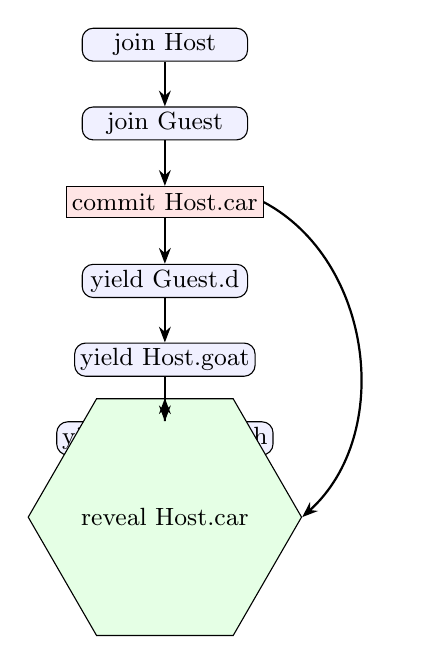
\begin{tikzpicture}[
  every node/.style={font=\small},
  ev/.style={draw, rounded corners, inner sep=2pt, minimum width=2.1cm,
             minimum height=4mm, fill=blue!6},
  cnode/.style={draw, inner sep=2pt, minimum width=2.1cm, minimum height=4mm,
             fill=red!10},
  rv/.style={draw, regular polygon, regular polygon sides=6,
             inner sep=0pt, minimum width=2.3cm, minimum height=5mm,
             fill=green!10},
  arr/.style={-{Stealth[length=2mm]}, thick},
]
\node[ev]    (j0) at (0,0)   {join Host};
\node[ev]    (j1) at (0,-1)  {join Guest};
\node[cnode] (c2) at (0,-2)  {commit Host.car};
\node[ev]    (y3) at (0,-3)  {yield Guest.d};
\node[ev]    (y4) at (0,-4)  {yield Host.goat};
\node[ev]    (y5) at (0,-5)  {yield Guest.switch};
\node[rv]    (r6) at (0,-6)  {reveal Host.car};

\draw[arr] (j0) -- (j1);
\draw[arr] (j1) -- (c2);
\draw[arr] (c2) -- (y3);
\draw[arr] (y3) -- (y4);
\draw[arr] (y4) -- (y5);
\draw[arr] (y5) -- (r6);
\draw[arr, bend left=55] (c2.east) to (r6.east);
\end{tikzpicture}
\end{center}

Two facts to read off this picture.  First, the long-distance
edge from \TT{commit Host.car} to \TT{reveal Host.car} captures
the commit-reveal pairing structurally: the reveal is enabled
only after every preceding move, including its own committed
predecessor.  In any configuration where the reveal is on the
frontier, every prior decision has been made.  Second, the data
dependency from \TT{yield Guest.d} to \TT{yield Host.goat} ---
because Host's guard reads \TT{Guest.d} --- is collapsed into
the phase-order edge, so it does not appear separately; the
guard read is redundant given the existing chain.

This is the typical shape of turn-taking games: a sequential
chain plus the structural pair for hidden information.
Concurrency-driven rewriting becomes interesting when several
roles share a single yield statement, as in the Vickrey example
treated in \S\ref{sec:commit-reveal}.

\subsection{Visibility-aware perfect recall}
\label{sec:eventgraph:visibility-recall}

For game-theoretic analysis, two players are in the same
information set at a node $B$ iff they have observed the same
sequence of public events leading to $B$.  In the EventGraph this
becomes a structural notion: the set of fields observable by role
$R$ at node $B$ is

\begin{equation*}
  \mathrm{obs}_R(B) \;=\; \bigl\{\, f \;\big|\; f \text{ is written by some predecessor } A \text{ of } B,
            \text{ and either } \mathrm{owner}(A) = R \text{ or } \mathrm{vis}(A,f) \in \{\PUBLIC, \REVEAL\} \bigr\}.
\end{equation*}

This is the projection used by the Gambit backend to compute
information sets and, in a closely related form, by the MAID and
Scribble backends.  An IR helper \TT{observableFieldsAt(B)}
computes it; the formula above is the only place where
observability is defined.

\subsection{Implementation notes}

The EventGraph class wraps a generic \TT{Dag<NodeId>} with the
per-node payload map and a precomputed reachability relation.
Reachability is computed once when the graph is built and reused
for all queries; building it eagerly is the right tradeoff in
this setting because the graph is small (forty-some nodes for
the largest example) and the queries are many
(\TT{reaches}, \TT{ancestorsOf}, \TT{canExecuteConcurrently}).

The constructor takes a node set, a per-node predecessor map, and
a per-node payload map, and returns either an EventGraph or
\TT{null}; the latter happens when an invariant is violated.
Three internal validators run inside the constructor:

\begin{itemize}\itemsep1pt
\item acyclicity, via topological sort;
\item commit-reveal ordering, by checking that every \REVEAL has
  a matching \COMMIT among its ancestors;
\item read-visibility, by checking that every field appearing in a
  guard at node $B$ is either written \PUBLIC before $B$, or has
  been revealed before $B$, or is being written by $B$ itself.
\end{itemize}

The corresponding error in the frontend is a static error, with a
source span pointing back to the offending \TT{where} clause or
\TT{commit/reveal} pair.  This is the same set of checks a
human reviewer would perform when reading a hand-written
commit-reveal contract --- the IR just performs them
systematically.

A note on the read-visibility check: in addition to fields written
\PUBLIC or revealed by a predecessor, the validator also accepts a
guard read of a field that the actor itself committed earlier on
the same DAG path.  An owner ``sees their own writes'' is therefore
a slightly stronger statement than the bullet above admits: it
includes their own \emph{committed} fields as well as the
public/revealed ones.  In practice the typechecker's pre-IR
desugaring strips fields written by the current node from the
guard's scope, so this branch matters mostly for guards that
reference an actor's earlier private writes.

\section{Automatic Commit-Reveal Insertion}
\label{sec:commit-reveal}

This section describes the EventGraph rewrite that protects
simultaneous public moves from transaction-ordering adversaries.
The pass is small but the property it secures is one of the most
visible payoffs of using Vegas: a programmer who writes
``two players \TT{yield} simultaneously'' gets the commit-reveal
protocol the textbook would have insisted on, deployed on chain
with no further work.

\subsection{The problem}
\label{sec:cr:problem}

Consider the two-line specification
\begin{lstlisting}[style=vg]
yield A(x: bool);
yield B(y: bool);
\end{lstlisting}
At the EventGraph level these are two PUBLIC writes on concurrent
nodes.  Read as a game, the analysis is unambiguous: A and B move
simultaneously without observing each other.  Read as a Solidity
contract, the implementation has to be cautious.  If A's
transaction is in the public mempool, B can read \TT{x} before
deciding \TT{y}.  An ordering adversary (a builder, or a competing
searcher) can promote the read-then-write transaction.  The
specification's notion of simultaneity is broken by the deployment
target's notion of transaction ordering.

This is a specific subclass of MEV --- \emph{observation-before-action}
on simultaneous moves --- and the canonical mitigation is well
known~\citep{Blum1983CoinFlipping,Pedersen1991Commitment,breidenbach2018enter}:
each role first commits to a hash of their move, and only after
all roles have committed does anybody reveal.  Vegas applies the
mitigation automatically, by rewriting the EventGraph.

\subsection{Risk partners}

Two nodes are \emph{risk partners} when both are pure-public
writes, neither reaches the other in the dependency DAG, and they
are distinct.  This is precisely the configuration in which the
ordering adversary problem arises.  The pass identifies the set
of nodes that have at least one risk partner --- call this set
$\mathrm{Split}$ --- and rewrites every node in $\mathrm{Split}$.

Pure-public writes (every visibility tag is \PUBLIC) are the only
candidates for rewriting.  Nodes that already commit (visibility
\COMMIT) need no rewriting; their reveal partner is already
present.  Nodes that themselves have a guard reading another
actor's private value cannot arise (the typechecker rejects such
reads).  And nodes that are in a strict dependency relation with
their potential partner are not concurrent, so the ordering
adversary has no informational asymmetry to exploit.

\subsection{The rewrite}
\label{sec:cr:rewrite}

For each $a \in \mathrm{Split}$ the pass introduces two fresh
nodes:

\begin{itemize}\itemsep1pt
\item a \emph{commit node} $a^{c}$, replacing $a$ as the new owner
  of the deposit (if $a$ was a \TT{join} step) and of the
  original predecessors of $a$, but with all of $a$'s \PUBLIC
  writes retagged as \COMMIT and with a trivial guard
  (anything is allowed to commit);
\item a \emph{reveal node} $a^{r}$, carrying $a$'s original guard,
  with all the same writes retagged as \REVEAL.
\end{itemize}

Edges are wired so that

\begin{itemize}\itemsep1pt
\item $a^{c}$ has the same predecessors $a$ originally had;
\item $a^{r}$ has predecessors $\{a^{c}\} \cup \{b^{c} : b \in
  \mathrm{partners}(a)\} \cup \mathrm{pred}(a)$;
\item every node that previously depended on $a$ now depends on
  $a^{r}$ instead.
\end{itemize}

The second clause is the informational barrier: $a^{r}$ cannot
fire until \emph{all} of $a$'s risk partners have also committed.
After the rewrite, no \REVEAL node is on the frontier of any
configuration in which a sibling \COMMIT is still unresolved.
\Cref{sec:eventgraph:frontier} called this the structural
information barrier; the rewrite is what guarantees it for any
group of originally-simultaneous public moves.

\subsection{Illustration}

The bidder fragment of the Vickrey auction
(\S\ref{sec:lang:vickrey}) is the cleanest case.  The source

\begin{lstlisting}[style=vg]
yield or split B1(b: bid) B2(b: bid) B3(b: bid);
\end{lstlisting}

produces, before the rewrite, three concurrent \PUBLIC nodes
(left) and after the rewrite, three commit nodes followed by three
reveal nodes that all wait for the full commit phase (right).

\begin{center}
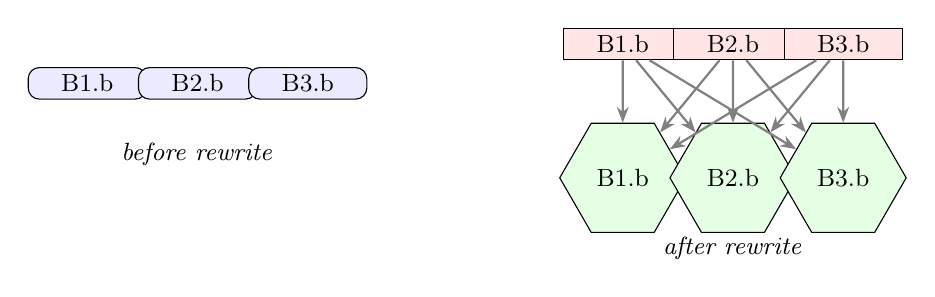
\begin{tikzpicture}[
  every node/.style={font=\small},
  pu/.style={draw, rounded corners, inner sep=2pt, minimum width=1.5cm, minimum height=4mm, fill=blue!8},
  cnode/.style={draw, inner sep=2pt, minimum width=1.5cm, minimum height=4mm, fill=red!10},
  rv/.style={draw, regular polygon, regular polygon sides=6, inner sep=0pt,
             minimum width=1.6cm, minimum height=5mm, fill=green!10},
  arr/.style={-{Stealth[length=2mm]}, thick}
]
\node[pu] (b1) at (-0.8, 0)   {B1.b};
\node[pu] (b2) at ( 0.6, 0)   {B2.b};
\node[pu] (b3) at ( 2.0, 0)   {B3.b};
\node     at ( 0.6,-0.9) {\textit{before rewrite}};

\node[cnode] (c1) at ( 6.0, 0.5) {B1.b};
\node[cnode] (c2) at ( 7.4, 0.5) {B2.b};
\node[cnode] (c3) at ( 8.8, 0.5) {B3.b};
\node[rv] (r1) at ( 6.0,-1.2) {B1.b};
\node[rv] (r2) at ( 7.4,-1.2) {B2.b};
\node[rv] (r3) at ( 8.8,-1.2) {B3.b};
\node     at ( 7.4,-2.1) {\textit{after rewrite}};
\foreach \c in {c1, c2, c3}
  \foreach \r in {r1, r2, r3}
    \draw[arr, gray] (\c) -- (\r);
\end{tikzpicture}
\end{center}

After the rewrite, each bidder's reveal depends on every bidder's
commit.  Reading off the new graph: no reveal is enabled on a
frontier where any commit is missing, so no bidder learns another
bidder's value before they themselves have committed.

\subsection{What changes for the backends}

Every backend sees the rewritten graph, not the original.  The
operational backends (Solidity/Vyper) therefore emit a
commit-then-reveal pair of contract functions per rewritten
action; the Solidity backend uses the hidden write's payload as
the input to a hash and stores the hash, then on reveal verifies
the hash and assigns the public field.  The Gambit backend reads
the rewritten graph as a sequence of two simultaneous-move rounds
(commits, then reveals); information sets are computed from the
new graph in the usual way, and they correctly reflect the
informational barrier.  No backend-specific commit-reveal logic
exists: the property is paid for once, in the IR, and consumed
everywhere.

\subsection{What the rewrite does \emph{not} do}

A few caveats.

\paragraph{Cryptographic strength is not the IR's concern.}  The
rewrite stipulates \emph{that} a hidden value is committed before
the public reveal; it does not specify the cryptographic primitive.
The Solidity backend chooses a domain-separated keccak with a
random salt and a per-game tag; a different backend (Bitcoin) uses
its native opcodes.  The choice is the backend's; the IR-level
property holds for any binding, hiding commitment.

\paragraph{The rewrite does not address adaptive adversaries
elsewhere.}  An adversary can still censor a player's transaction
to force a timeout; the bail-out subgame (\S\ref{sec:liveness})
makes this a strategic choice with explicit payoff, so the game
model sees it, but censorship-resistance per se is not what the
commit-reveal pass provides.

\paragraph{The rewrite does not enlarge the set of safe
patterns.}  Only \emph{originally-concurrent} public writes are
rewritten.  A public write that is in strict order with all other
public writes is not at risk and stays a single node.  This is
intentional: there is no point in adding round-trips for moves
that the dependency relation already serialises.

\subsection{The information-barrier property}
\label{sec:cr:barrier}

What the rewrite produces is a graph in \emph{commit-reveal
normal form}: every node whose original write was concurrent
with another's has been split into a commit-then-reveal pair,
and every reveal in the result is dominated in the DAG by all
of its risk partners' commits.  The strategic property the
rewrite delivers is the \emph{information barrier}: in any
configuration of the rewritten graph, no reveal node is on the
frontier while any of its commit prerequisites --- its own or a
risk-partner's --- is still unresolved.

Stated informally for the rewritten graph $G$:
\begin{quote}\itshape
For every reveal node $r$ and every configuration $C$ of $G$
with $r$ enabled in $C$, every node $c \in \mathrm{commitPred}(r)$
has been assigned in $C$.
\end{quote}
By the construction of the rewrite this holds: each
$r = a^r$ has $\{a^c\} \cup \{b^c : b \in \mathrm{partners}(a)\}$
among its predecessors, so $r$ can only be enabled when every
named commit is done.

The same property is proved as a theorem in the companion Lean
library VegasCore as the ``Commit/reveal information barrier''
result over the canonical event graph
(\S\ref{sec:vegascore:theorems}): any event graph in which
commits dominate reveals satisfies the barrier, regardless of
how it was obtained.  Vegas's rewrite produces such graphs from
not-yet-canonical input; VegasCore certifies that any such graph
satisfies the barrier.

\subsection{Implementation}

The rewrite lives at \file{ir/EventGraph.kt} as a static method
\TT{expandCommitReveal} on the \TT{EventGraph} class.  It runs
once, immediately after the initial IR construction, before any
backend reads the graph.  The implementation is roughly sixty
lines of Kotlin and is reachability-driven: it iterates over the
existing nodes, builds the risk-partner relation by checking
$\neg(\mathrm{reach}(a,b) \vee \mathrm{reach}(b,a))$ for each
pair of pure-public nodes, and then performs the local rewrite
for each risk-partner-bearing node, allocating fresh node ids
above the current maximum.  The resulting graph is re-validated
by the EventGraph constructor (it must still be acyclic, the new
\COMMIT-\REVEAL pairs must be in order, and the read-visibility
discipline must be preserved).  The post-rewrite validation is
mostly defensive: all three properties are preserved by the
local rewrite construction, and the barrier property of
\S\ref{sec:cr:barrier} is preserved transitively.

\section{The Solidity and Vyper Backends}
\label{sec:solidity}

The EVM backends translate the EventGraph into a deployable smart
contract.  Both languages target the same compilation pass via a
shared EVM intermediate representation (\TT{evm.EVMIR}); only the
final pretty-printer differs.  This section walks through the
Solidity output and notes the few divergences for Vyper.  We are
careful to describe the actual generated code, not an idealised
version of it: the bail-out mechanism in particular is simpler than
the language-level story might suggest, and a few of its
consequences belong in the open-questions list rather than the
guarantees list.

\subsection{Threat model}
\label{sec:solidity:threats}

The compiled contract is meant to survive a transaction-ordering
adversary --- a builder or competing searcher who can choose which
pending transactions to include and in what order --- and to remain
liveness-preserving when a participant stops responding.  It is not
designed against:

\begin{itemize}\itemsep1pt
\item \emph{Censorship.}  An adversary who indefinitely excludes a
  participant's transactions is modeled as forcing a timeout, which
  marks the participant as \TT{bailed} and triggers the language-level
  quit handler.
\item \emph{Cross-contract interactions.}  The contract is a closed
  system; no calls into other contracts are emitted (the only
  outbound action is a direct ETH transfer to a registered
  participant address during withdrawal).
\item \emph{Gas-cost games.}  Gas is a real-world cost that affects
  which moves are rational, but the analytical backends ignore it.
  Bounded per-action gas envelopes (e.g.\ via
  GASTAP~\citep{Albert2020Gastap}) would be needed to bring gas into
  the strategic model; this is planned but not implemented.
\item \emph{Cryptographic primitives.}  The contract relies on
  keccak-256 being binding and hiding.  Domain separation and
  per-deployment binding are in the hash composition
  (\S\ref{sec:solidity:commit-reveal}), but the strength of the
  primitive itself is taken as given.
\end{itemize}

The remainder of this section describes the construction; the
``honestly imperfect'' parts of the design (especially the single
global timeout window) are flagged inline.

\subsection{Storage layout}

The contract's storage is derived directly from the EventGraph.
There are five families of slots.

\paragraph{Per-node completion.}  A two-level mapping
\TT{actionDone[role][actionId]} records, for each role and each
node, whether the node has fired.  A symmetric mapping
\TT{actionTimestamp[role][actionId]} stores the block timestamp at
which it fired.  Node ids are integers assigned by a deterministic
topological linearisation of the EventGraph; one
\TT{uint256 constant ACTION\_\textit{Role}\_\textit{n}} is emitted
per node.  The integer \TT{\textit{n}} is the node's source position
(making the constant name human-readable), while the assigned
constant \emph{value} is its topological index.

\paragraph{Role registry.}  A mapping
\TT{roles[address] => Role} associates EOAs with the roles they
have joined, and a per-role \TT{address\_\textit{Role}} slot
stores the registered address.  A small \TT{enum Role} carries one
constructor per role plus a \TT{None} sentinel.

\paragraph{Game state.}  For each \emph{written field} in the
EventGraph the contract stores the field's value.  A field with
\PUBLIC visibility uses a slot of the field's native type
(\TT{int256}, \TT{bool}, etc.); a field with \COMMIT visibility
uses a separate \TT{bytes32} slot for the commitment hash, with the
revealed value filled in by the matching reveal action.  Each
value slot is shadowed by a \TT{done\_\textit{slot}: bool} flag.

\paragraph{Per-role bookkeeping.}  Three booleans per role:
\TT{done\_\textit{Role}} (the role has joined),
\TT{claimed\_\textit{Role}} (the role has claimed its terminal
payout), and a private \TT{bailed[\textit{Role}]} (the role has been
marked inactive after a timeout).

\paragraph{Game-wide constants.}  A constant \TT{TIMEOUT} sets the
inactivity window, in seconds (the default is 24 hours).  A
constant \TT{COMMIT\_TAG} (a hashed domain-separation tag) and the
contract's deployed address are folded into every commitment hash.

\subsection{Modifiers and the depends pattern}
\label{sec:solidity:depends}

The contract has no global step counter.  Each per-node function is
guarded by a \TT{depends} modifier per predecessor.  The modifier
itself does two things: it advances the contract's
inactivity-timeout state (potentially marking some role
\TT{bailed}), and it conditionally requires the predecessor to have
completed.  Read top to bottom:

\begin{lstlisting}[style=sol]
modifier depends(Role role, uint256 actionId) {
    _check_timestamp(role);
    if (!bailed[role]) {
        require(actionDone[role][actionId], "dependency not satisfied");
    }
    _;
}
\end{lstlisting}

The body invokes \TT{\_check\_timestamp(\textit{role})}, which marks
\TT{\textit{role}} as \TT{bailed} iff the current
\TT{block.timestamp} exceeds a shared global high-water mark
\TT{lastTs} by more than \TT{TIMEOUT}; otherwise it leaves the
state unchanged.  If \TT{\textit{role}} is not bailed, the
predecessor's completion flag is required; if it is bailed, the
\TT{require} is skipped and the dependent action proceeds.  Two
additional modifiers complete the gating: \TT{action(role, id)}
asserts that the action has not yet fired, marks it done, runs the
body, and updates \TT{actionTimestamp} and \TT{lastTs};
\TT{by(role)} asserts that the calling EOA holds the given role
and is not itself bailed.

A typical per-node function looks like:

\begin{lstlisting}[style=sol]
function move_Guest_3(int256 _d)
    external
    by(Role.Guest)
    depends(Role.Host, ACTION_Host_0)
    depends(Role.Guest, ACTION_Guest_1)
    depends(Role.Host, ACTION_Host_2)
    action(Role.Guest, ACTION_Guest_3)
{
    require(_d >= 0 && _d <= 2, "domain");
    Guest_d = _d;
    done_Guest_d = true;
}
\end{lstlisting}

Every emitted action is named \TT{move\_\textit{Role}\_\textit{n}}
where \textit{n} is the source position.  The function's dependency
list is exactly the predecessor set of the node in the EventGraph
(after the commit-reveal expansion).  Concurrent nodes share the
prefix of the chain up to the divergence point and are otherwise
free to be called in any order.

\subsection{Commits and reveals}
\label{sec:solidity:commit-reveal}

Every COMMIT-tagged write becomes a function that takes a
\TT{bytes32} commitment and stores it; every REVEAL-tagged write
takes the cleartext value plus a salt, recomputes the commitment,
and asserts equality with the stored hash before performing the
public write.  The commitment hash is composed as

\begin{equation*}
  \mathit{keccak256}\bigl(
    \mathrm{abi.encode}(
      \textsc{COMMIT\_TAG},\
      \mathrm{address(this)},\
      \mathrm{role},\
      \mathrm{actor},\
      \mathit{keccak256}(\mathrm{payload})
    )
  \bigr).
\end{equation*}

The pieces serve distinct roles.  The \texttt{COMMIT\_TAG} provides
cross-protocol domain separation.  \TT{address(this)} ties the
commitment to this particular deployment, preventing replay across
copies of the same protocol.  The \TT{role} identifier defends
against role-swapping replays within a single deployment; the
\TT{actor} address binds the commitment to the EOA that posted it.
The payload is pre-hashed before being folded in, so the outer
hash works over a fixed-size input regardless of the parameter
list.

Vyper emits the analogous construction using the language's
\TT{assert} idiom and slightly different storage syntax.  The
generated bytecode is comparable.

\subsection{The single-window timeout and its consequences}
\label{sec:solidity:bail}

The timeout mechanism is simpler than the language-level story
might suggest, and it is worth describing exactly.

The contract maintains a single global \TT{lastTs} slot, updated to
\TT{block.timestamp} on every successful action.  Whenever a
modifier is entered, \TT{\_check\_timestamp(role)} is called: if
\TT{block.timestamp > lastTs + TIMEOUT}, the named role is marked
\TT{bailed} \emph{and} \TT{lastTs} is reset to the current
timestamp.  In effect, the contract has one sliding inactivity
window shared across all participants: if no action has happened
anywhere for \TT{TIMEOUT} seconds, the next caller can mark
\emph{some} role as bailed and the window restarts.

This has two non-obvious consequences worth flagging:

\begin{itemize}\itemsep1pt
\item \emph{The role that gets marked is the role named in the
  caller's modifier.}  \TT{depends(Role.Host, \ldots)} on a window
  expiry marks \TT{Host} as bailed; \TT{by(Role.Guest)} on a window
  expiry marks \TT{Guest}.  This is approximately right --- the
  function call points at a role expected to have acted --- but it
  is not the same thing as ``the unique unresponsive role''; the
  attribution is structural rather than analytical.
\item \emph{Bail is one-way.}  Once \TT{bailed[\textit{R}] = true},
  the \TT{by(R)} modifier rejects any subsequent action from
  \TT{R}.  A role that goes offline briefly and reconnects after
  the window expires has lost the right to play.  The
  language-level treatment of \TT{Quit} as a definitive move is the
  source of this design; it is operationally simple, but it does
  mean that a fair-playing role with a flaky connection is at risk
  in long protocols.
\end{itemize}

When a dependent action runs against a bailed predecessor, the
\TT{depends} modifier skips its \TT{require}, but it does \emph{not}
fabricate writes for the missing fields.  Their value slots and
their \TT{done\_} flags remain in their default state (zero, and
\TT{false} respectively).  Downstream code that needs to
distinguish ``never written'' from ``written to the default value''
relies on the language's \TT{opt T} typing: a field declared with
an \TT{or null} handler is typed \TT{opt T}, and the \TT{withdraw}
clause is required to inspect its \TT{done\_} flag.

The fair-play guarantee one would like --- ``every role can drive
the contract from any reachable configuration to a terminal
allocation'' --- is plausible for protocols whose \TT{withdraw}
clause is total on the public state (including \TT{done\_} flags),
but it is not proved.  Stating and proving it under the explicit
execution model is the central refinement-theorem target of the
ongoing VegasCore work; today, the test suite checks that the
\TT{withdraw} clause type-checks against the optional fields it
must handle, and that hand-played example traces reach a terminal
allocation, but no machine-checked proof is shipped.

\subsection{Withdraw and payout}

The terminal \TT{withdraw} clause is compiled into one entry
point per role.  Each role calls its own
\TT{withdraw\_\textit{Role}()} to receive their share, guarded by
a \TT{claimed\_\textit{Role}} flag to prevent double-payment.  The
payout expression is lowered to EVM IR by direct structural
translation; the body computes the expression against the public
state (including \TT{done\_} flag inspection for optional fields)
and transfers the resulting amount to the role's stored address
using a low-level \TT{call} with the computed value.

Conservation is checked statically against the deposit total
during compilation (symbolic checks where possible; exhaustive
enumeration for the finite-type case).  The contract therefore
does not need to verify at runtime that all role payouts sum to
the pool.

\subsection{Things the backend deliberately leaves alone}

Several real concerns are not addressed by the Solidity emission
because they are scoped out of the language.  Gas costs as a
strategic factor; mempool-level censorship beyond what the bail
mechanism handles; cross-contract interactions and oracle reads;
admin keys, upgrade proxies, and pausable patterns.  Each is a
deliberate restriction in the same vein as the language's
bounded-types-only stance: drawing the boundary tightly is what
makes the analytical backends' outputs faithful to the deployed
code, and what makes ``the same source for two views'' a defensible
claim.

\section{The Gambit Backend}
\label{sec:gambit}

The Gambit backend turns the EventGraph into an extensive-form game
in Gambit's \TT{.efg} format~\citep{McKelveyMcLennanTurocy2006Gambit}.
Once written, the file can be loaded directly into Gambit (or
OpenSpiel~\citep{LanctotEtAl2019OpenSpiel}, via standard adapters)
to compute Nash equilibria, dominant strategies, or any other
property Gambit knows how to check.  This section describes how the
backend constructs the tree from the graph.

\subsection{Frontier exploration}

The backend is a depth-first frontier expander.  At a configuration
$C$, it enumerates the frontier, groups its nodes by owning role,
and for each role that has at least one node on the frontier it
generates a Gambit decision node.  Multiple roles may have nodes on
the same frontier; these are simultaneous moves in the strategic
analysis (\S\ref{sec:eventgraph:frontier}).  Gambit's \TT{.efg}
format does not have a primitive simultaneous block: the backend
nests the per-role decision nodes in a canonical role order and
arranges the information sets so that each role's information set
hides the other roles' choices at the same strategic move.  The
strategic content is in the information sets, not the textual
nesting order.

For each role, the actions are the products of values its nodes may
take.  Bounded-type fields have an explicit finite alphabet
(e.g.\ \TT{door = \{0,1,2\}} has three values); the \TT{Quit} move
is added as an extra alphabet symbol when the role's node has a
quit handler.  A node performing a hidden commit has its commit
parameter listed as ``Hidden(\textit{value})'' rather than the
cleartext value: from the perspective of the game, the value
matters but the observer does not see it.  When the corresponding
reveal node fires, the resolved value collapses ``Hidden(\dots)''
to a concrete number.

For each combination of role moves at the current frontier, the
backend computes the resulting configuration, recurses, and emits
the subtree.  When the frontier is empty --- the configuration has
finished every node --- the \TT{withdraw} clause is evaluated to
produce a terminal node carrying the payoff vector.

\subsection{Information sets}

A player's information set at a decision node is the set of
histories they cannot distinguish, given what they have observed.
The backend computes this directly from
$\mathrm{obs}_R(B)$ (\S\ref{sec:eventgraph:visibility-recall}):
two Gambit decision nodes are in the same information set for
role $R$ iff the projections of their pre-state to
$R$-observable fields are equal.

In practice, hidden commits create the information sets that
matter.  In the Vickrey example, each bidder's reveal node is at a
depth where the other bidders' commitments have fired but their
values have not been revealed; the reveal node therefore sits in
an information set whose members differ only in the other
bidders' hidden values.  This is the correct strategic
representation of a sealed-bid auction.

\subsection{Pruning}

Two reductions are run on the produced tree before emission.

\emph{Unreachable subtrees are dropped.}  When a guard rules out a
move (the guard evaluates to false for the would-be combination of
values), no edge is emitted; this is straightforward as long as
the guard's free variables are all evaluated at the decision
node's information set.

\emph{Trivial continuations are collapsed.}  When a player has
exactly one legal move at a decision node (often because
\TT{Quit} is the only choice on a degenerate branch), the
backend emits a single edge and proceeds.  This keeps the tree
size manageable on examples with many forced timeouts.

\subsection{Limits}

A few characteristics of the backend should be acknowledged.

\paragraph{Tree size blows up with the type universe.}  The
backend enumerates the cross-product of move alphabets at each
frontier.  For a hypothetical three-bidder auction with 11-value
bids and a quit option, the commit frontier alone yields
$12^3 = 1728$ branches (where the strategic choice actually
happens); each reveal node only branches by 2 (the committed
value or Quit), but the reveal frontier is visited once per
commit combination, so the total tree size grows
multiplicatively.  The bundled Vickrey example uses a 3-value
bid type to keep the tree analysable.  This is a limit of
tree-enumeration analysis, not of the language: a Vegas
program with a larger bid type compiles and deploys correctly,
but the resulting EFG becomes too large for Gambit-style
equilibrium search, and the analyst gains nothing from the EFG
backend past that point.  This is fine for the example library;
it is not what one would deploy against a competitive-bidding
mechanism with millions of bid levels.  Vegas's contract-side bid types are typically narrow because
Gambit cannot otherwise analyse them; wider ranges deploy fine
but make Gambit-side analysis infeasible.  This is the explicit
tradeoff in carrying both views in the same source.

\paragraph{Move alphabets must be bounded.}  An action whose
parameter has type \TT{int} is rejected by the Gambit backend at
compile time.  The Solidity backend has no such restriction (it
stores an \TT{int256} directly); the Gambit constraint is
enforced via a per-backend disable list in the test harness.

\paragraph{Quit appears as a real move.}  Because the bail-out
subgame is a strategic option in Vegas's semantics, the
\TT{.efg} contains a \TT{Quit} branch wherever the source action
has an or-handler.  This is the right thing
game-theoretically (it captures the strategic option of timing
out), but it does inflate the tree.

\paragraph{Chance nodes.}  Actions owned by a chance label ---
a \TT{random} role or a \TT{sample} binding --- are emitted as
Gambit chance moves.  Each parameter carries a per-node
distribution: either the explicit \TT{$\sim$ uniform/weighted}
annotation declared at the parameter, or the inferred uniform
over the parameter's bounded domain when no annotation is
present.  A self-only guard on the chance action is interpreted
as standard probabilistic conditioning: the guard-surviving
support is renormalised so that probabilities sum to one on the
children of the chance node.  Contextual guards (referring to
prior fields) are conditioned per trace, with a fresh
renormalisation at each reached context.  Each chance event is
a node of its own, with the same simultaneous-move treatment as a
player move.

\section{Other Backends}
\label{sec:other-backends}

Past the EVM and Gambit backends, the rest of the family share the
EventGraph but address different consumers: a constraint solver
(SMT-LIB), a session-typed protocol checker (Scribble), a Bitcoin
Lightning channel (for the two-party fragment), a MAID exporter
(for the Thrones game-theory workbench), a GraphViz visualisation,
and a Coq/Lean deep embedding of the protocol as a dependent
typing problem.  Each is short enough to cover in one section.

\subsection{SMT-LIB}

The SMT backend (\file{backend/smt/Smt.kt}) encodes the EventGraph
as a set of quantifier-free constraints over per-node ``done''
flags and per-field value variables.  A bounded-type field is a
finite-sort variable; a guard is its boolean lowering;
dependencies become implications
\(\mathit{done}_B \Rightarrow \bigwedge_{A \in \mathrm{pred}(B)} \mathit{done}_A\).
Reachability queries are written as additional constraints
asserting that a chosen role gets a payoff at least $x$.

The result is given to Z3 (or any SMT-LIB-2 solver) for
satisfiability.  Two principal uses:

\begin{itemize}\itemsep1pt
\item \emph{Witness searches.}  ``Is there a play that gives role
  $R$ a payoff $\geq c$?''  A satisfying assignment is a concrete
  history.
\item \emph{Coalition queries.}  A DQBF encoding is also generated,
  in which a chosen coalition's variables are existentially
  quantified and the complement's are universally quantified.  The
  resulting formula is true iff the coalition has a strategy that
  achieves a property against any response.  This is a coarse
  analogue of best-response analysis useful for sanity checks on
  small examples.
\end{itemize}

Z3 is fast on the example library; the encoding is plain enough
that it is also useful as a sanity-check on the IR (a guard that
nobody can ever satisfy will show up as a falsifying constraint).

\subsection{Scribble}

Scribble~\citep{HondaYoshidaCarbone2008MPST} is a session-types
implementation that records the legal sequencing of messages in a
multi-party protocol.  The Scribble backend
(\file{backend/scribble/}) projects the EventGraph onto the
public-message subset --- skipping commits, retaining reveals and
public yields, dropping internal randomness --- and emits a global
type whose sequencing is the topological order of the public
frontier.  Recursion in the produced Scribble protocol is empty
(the protocol is acyclic by construction).

The output is useful to anyone who wants a static check that
their off-chain client library is sending messages in the right
order; Scribble's projection toolchain can derive per-role local
types from the global protocol.

\subsection{Bitcoin / Lightning (sketch)}

A proof-of-concept backend (\file{backend/bitcoin/}) targets the
two-party Lightning channel for the subset of Vegas games with
exactly two strategic roles.  Each EventGraph node is mapped to
a state in a Bitcoin script state machine; commitments use
\TT{OP\_HASH160} and \TT{OP\_EQUAL}, with state transitions
encoded as signed updates of the channel's commitment
transaction.  The output is a textual transcript of the
Lightning protocol moves needed to realise the game --- not a
deployable artifact.  Deployment on a real Lightning node, and
the integration work that would entail, is out-of-band.

Its value here is the existence proof: the EventGraph
abstraction lifts to a non-EVM execution layer with completely
different cryptographic primitives, with no change to the IR.
A proper Bitcoin/Lightning backend is on the future-work list,
not a claim of the present work.

\subsection{MAID}

MAID~\citep{koller2003multi} (Multi-Agent Influence Diagrams)
factor a multi-agent decision problem into decision nodes,
chance nodes, utility nodes, and the conditional probability
distributions that wire them together.  Vegas can emit a MAID
suitable for the Thrones game-theory workbench.

The MAID backend has a real expressiveness limit.  In plain
MAIDs, a decision node's action set is a single static domain;
there is no place to say ``the legal action set depends on the
parents' values''.  A Vegas guard like
\TT{where Host.goat != Guest.d} has nowhere to go in such a
MAID: the encoding would silently drop the constraint and present
the Host as being able to pick any door.  The current MAID
emitter therefore refuses to emit for any game whose guards
reference fields written by other nodes; it accepts self-only
guards (a guard that only constrains the value being written) but
does not yet narrow the resulting MAID node's domain.  Both
narrowing self-only guards and supporting context-dependent
domains in some MAID extension are listed in \file{TODO.txt}.

Where MAID does apply --- protocols with trivial or self-only
guards --- the MAID view is more compact than the unfolded
extensive-form tree.  For the rest, Gambit's EFG is the more
expressive target.

\subsection{Coq / Lean: Diamond DAG witness records}
\label{sec:other:diamond}

The Gallina (Coq) and Lean~4 backends emit a deep embedding of
the EventGraph as a dependently-typed family of records.  The
encoding is worth describing directly: every move and every
guard is a type-level proof obligation, and player strategies
become functions on typed prior witnesses.

For an EventGraph with $n$ nodes, the backend emits a chain of
records $W_0, W_1, \dots, W_n$, where $W_i$ is the (typed) state
after the first $i$ nodes have fired.  Each $W_i$ is parameterised
on the entire history $W_0, \dots, W_{i-1}$, with fields:

\begin{itemize}\itemsep1pt
\item one named field per parameter written by node $i$, of the
  parameter's bounded type, with the field name embedding the
  parameter and owning role (e.g.\ \TT{hidden\_car\_Host} for a
  committed value, \TT{d\_Guest} for a public yield);
\item one proof field per guard ---
  \TT{$W_i$\_guard\_domain\_\textit{f}} for the domain restriction
  and \TT{$W_i$\_guard\_logic} for the user-supplied \TT{where}
  clause;
\item for reveals, a proof
  \TT{$W_i$\_guard\_reveal\_\textit{f}} that the revealed value
  equals the value committed in an ancestor witness;
\item nothing else.
\end{itemize}

The backend emits one of two top-level records, named for the
side of the protocol they encode.  \TT{ActionDag} is the
\emph{fair-play structure}: an inhabitant is a complete play of
the protocol together with proofs of every guard, every domain
restriction, and every reveal-matches-commit equation.  Inhabiting
\TT{ActionDag} is therefore the same as exhibiting that a fair
play exists.  \TT{EventDag} is the \emph{trace structure}: an
inhabitant is a realised history, with hidden fields wrapped in a
\TT{Maybe}-style carrier so that traces can be partially observed.
Actor strategies are functions from the prior witnesses
$W_0, \dots, W_{i-1}$ (projected to the actor's view) into the
appropriate field of $W_i$, with proofs --- so the encoding
captures \emph{at the type level} that every move is legal and
every reveal matches its commit.

The Coq and Lean backends each take a policy flag selecting which
records to emit:

\begin{itemize}\itemsep1pt
\item \TT{FAIR\_PLAY} (\TT{lean-fair} / \TT{gallina-fair}) emits
  \TT{ActionDag} only.  Every guard becomes a runtime
  \TT{decide}/\TT{rfl} obligation in the appropriate $W_i$.
\item \TT{INDEPENDENT} (\TT{lean-independent} /
  \TT{gallina-independent}) emits \TT{EventDag} only, with
  hidden fields wrapped in a \TT{Maybe} carrier and an
  \TT{isPresent} discipline on reveals.
\item \TT{MONOTONIC} (\TT{lean-monotone} / \TT{gallina-monotone})
  emits both records, with monotonicity guards
  (\TT{$W_i$\_guard\_have\_$w_j$}) certifying that prior commits
  remain valid for later reveals.
\end{itemize}

Each policy is exercised against the same example set in the
golden-master harness.

The Diamond DAG encoding is independent of the companion
VegasCore Lean library described in \S\ref{sec:vegascore}.  The
two coexist as different approaches to ``the same protocol viewed
through a proof assistant'': Diamond DAG ships a standalone
per-program object whose inhabitation is a witness; VegasCore is
a reusable library of definitions and theorems.  A third Lean
backend, emitting a Vegas program as an instance of VegasCore's
\TT{WFProgram} type, is planned (and listed in
\file{TODO.txt}) to bridge the two.

The encoding is interesting for two reasons.  First, it is
self-contained: the Lean object can be passed to a theorem
prover without depending on a large semantics library; the
encoding \emph{is} the semantics.  Second, because each step is
a function on prior witnesses, the player's choice schedule
appears as a strategy in the strict type-theoretic sense --- an
inhabitant of a function space whose codomain is pinned by
domain and where-clause proofs.  This view is closer to the
IF-logic and compositional-game-theory style of game
semantics~\citep{HintikkaSandu1989,GhaniHedgesWinschel2018CGT}
than to the state-machine view that Gambit's tree presents.

\subsection{GraphViz}

The simplest backend: a textual DOT description of the EventGraph
for debugging and presentation.  Player nodes are boxes; chance
roles are diamonds.  Visibility is encoded in fill colour: pink
for \COMMIT writes, green for \REVEAL writes, light grey for
\PUBLIC writes.  Useful for inspecting the result of the
commit-reveal expansion pass.

\section{Liveness and Quit Handlers}
\label{sec:liveness}

Vegas treats the operational question of \emph{what happens when
someone stops responding} as part of the surface syntax rather
than as an implementation detail.  This section walks through the
design: how the language exposes the choice to the programmer,
how the compiler realises it on the EVM, and where the model is
honest about its current limits.

\subsection{Why liveness is in the language}

A multi-party on-chain protocol is exposed to two kinds of
slow-or-absent participants: strategic ones (who decline to play
because the next move is not in their interest), and incapable
ones (client crashes, mempool censorship, gas exhaustion).  The
deployed contract has to decide what to do in both cases, and the
decision must be a total function of public history.  Vegas
makes that decision part of the source: every action that could
plausibly fail to occur carries an explicit handler:

\begin{lstlisting}[style=vg]
yield or split A(x: int);
\end{lstlisting}

The handler describes what the contract does, and the
game-theoretic analysis sees \TT{Quit} as a strategic move
available to the actor.  The two views agree by construction.

\subsection{The three group handlers}

A statement involving one or more roles in a single
\TT{yield}/\TT{commit}/\TT{reveal} group carries one of three
handlers.

\paragraph{split} The quitter's deposit is split among the
surviving roles (in a two-player game, the survivor gets it all).
This is the default for adversarial games: nobody profits by
walking out.

\paragraph{burn} The quitter's deposit is sent to a designated
burn address (or zero address, depending on chain conventions).
Useful in games where giving the deposit to surviving roles would
warp incentives --- voting schemes where a missing voter should
not enrich the others, for instance.

\paragraph{null} The missing field is treated as \TT{null} at the
typing level (the field's type becomes \TT{opt T}), the node's
\TT{done\_} flag is set by the contract, and the protocol
proceeds.  The \TT{withdraw} clause is required to handle the
optional case explicitly.  Useful for protocols where a
non-response is itself strategically meaningful (a delegate
failing to delegate).

\subsection{Per-query payoff handlers}
\label{sec:liveness:per-query}

A single multi-role statement sometimes needs different outcomes
depending on which role quit.  The language supports this via a
\TT{||} qualifier on the role's query:

\begin{lstlisting}[style=vg]
yield or split Bob(ok: bool) || { Alice -> 40 };
\end{lstlisting}

The right-hand side of \TT{||} is an \emph{outcome}: a payoff
allocation chosen from the same sublanguage that \TT{withdraw}
clauses use (a brace-block payoff, or \TT{split}/\TT{burn}/\TT{null}).
When the named role quits, the contract executes the handler's
outcome \emph{instead of} the rest of the protocol; control does
not return.  No subgame or callable game block is involved ---
the handler is a terminal allocation chosen at the bail point.

\subsection{Operational realisation}

The Solidity backend implements \TT{Quit} via a timeout-and-bail
mechanism (\S\ref{sec:solidity:bail}).  The contract maintains one
global inactivity window: if no action has happened anywhere for
\TT{TIMEOUT} seconds (default 24 hours), the next caller's
modifier marks the named role as \TT{bailed} and resets the
window.  Once bailed, the role's actions are rejected by the
\TT{by(Role)} modifier; the bail is one-way.

This single-window design is operationally simple and
implementable in a few lines of Solidity, but its attribution is
structural rather than analytical: it marks ``the role pointed at
by the modifier'' as bailed, not ``the role that was supposed to
act next''.  In a long protocol with several outstanding actions
in different roles, this attribution can be coarser than one would
ideally want.  A per-action deadline scheme would address this at
the cost of substantially more state; the current design is the
simpler starting point.

\subsection{Liveness in the game model}

For the Gambit backend, \TT{Quit} is an additional alphabet
symbol at every move site with a handler.  Equilibrium analyses
therefore see \TT{Quit} as a real move, with the payoff indicated
by the handler.  This is what lets the analysis surface griefing
incentives without modelling them outside the game.  In a
simultaneous \TT{or split} statement, for instance, \TT{Quit} is
strictly dominated by any non-quit move iff the split penalty
exceeds the worst non-quit payoff; the dominance check on the
generated EFG verifies the property mechanically.

\subsection{Limits today}

Two known limits worth flagging.

\paragraph{Fair-play liveness is not statically checked.}  A
\emph{fair-play guard} is a \TT{where} clause whose role can
always find a satisfying value, regardless of prior moves.  The
language does not verify that today; a contextual guard like
\TT{yield B(y: int) where y != A.x \&\& y != A.x + 1 \&\& y != A.x - 1}
over a type \TT{int = \{0..2\}} becomes unsatisfiable depending on
\TT{A}'s play, forcing \TT{B} to quit through no fault of its own.
The project's design notes sketch a static check
(exhaustive enumeration over bounded types, or an SMT call for
the general case) that would type the affected field as
\TT{opt T} when satisfiability cannot be established; implementing
it is on the TODO list under the name \emph{fair-play liveness}.

\paragraph{Computational tractability is not checked either.}  A
guard such as \TT{p * q == N} for a large semiprime \TT{N} is
satisfiable by definition but practically infeasible to satisfy.
Vegas treats this the same as a satisfiable guard; the player
will quit, the contract will bail, and the game model will
record that outcome via the handler.  No analysis distinguishes
``empty move space'' from ``intractable move space''.  This is
the standard limit of purely structural reasoning about action
availability.

\section{Connection to VegasCore}
\label{sec:vegascore}

A companion project, VegasCore, formalizes a core calculus over
the same event-graph carrier in Lean~4~\citep{deMouraUllrich2021,mathlib2020}.
The two artifacts are independent --- Vegas is a compiler tool;
VegasCore is a self-contained semantic construction --- but they
describe overlapping objects, and a programmer interested in
proving properties of a Vegas program will eventually want to
cross the bridge between them.  This section sketches the
correspondence, lists where the two diverge, and gives the gap
between today's state and a fully verified pipeline.

\subsection{What VegasCore is}

VegasCore is a Lean~4 library that formalizes the core
\TT{commit}/\TT{reveal}/\TT{sample}/\TT{let}/\TT{ret} calculus
underlying Vegas's source language.  Its central object is an
\TT{EventGraph} type elaborated from a checked program
(\TT{WFProgram}); the well-formedness conditions
--- visibility, freshness of binders, completeness of reveals,
normalization of sample distributions, and at-least-one-legal
action --- are statically encoded as fields of \TT{WFProgram}.
From a checked program VegasCore derives a probabilistic
\TT{Machine}, native strategy carriers, and kernel-game
presentations of the protocol; it states and proves frontier
commutation, the commit/reveal information barrier, agreement of
several outcome laws, a finite Kuhn realization theorem, and
backend-refinement transport.  All of this is mechanized in
Lean.

VegasCore's role in the project is to provide a
formally-mechanized referent for the kind of semantics that
Vegas's compiler informally implements.  Where Vegas's IR
constructor refuses to accept a graph violating the
visibility-on-reads invariant, VegasCore proves the corresponding
theorem about the elaborated graph; where Vegas's
commit-reveal-expansion pass produces an informationally
correct graph by construction, VegasCore proves frontier
commutation and the information barrier as theorems about the
abstract event graph.

\subsection{Shared vocabulary}

The two projects use the same names for the things they have in
common.  The list is short and almost exact:

\begin{center}
\begin{tabular}{ll}
\toprule
Vegas (this compiler) & VegasCore (Lean) \\
\midrule
EventGraph                  & EventGraph \\
node / nodeId               & event / node id \\
guard (\TT{scope}, \TT{expr}) & per-node guard $R$ \\
\COMMIT / \REVEAL / \PUBLIC writes & hidden + commit/reveal node kinds \\
frontier (\TT{FrontierMachine}) & frontier \\
\TT{random}                 & \TT{sample} \\
\TT{withdraw}               & \TT{Ret} \\
\bottomrule
\end{tabular}
\end{center}

For an entry-level reading of either project, this table is the
glossary: the Vegas reader who picks up the VegasCore chapter
already knows what an EventGraph is, and vice versa.

\subsection{Where they diverge, and why}

Each artifact has features the other does not.  The asymmetries
are deliberate.

\paragraph{Vegas surface keywords and macros.}  VegasCore's
surface language exposes the five core constructors directly;
Vegas's surface adds the user-facing
\TT{yield}/\TT{join}/\TT{commit}/\TT{reveal}/\TT{random}
keywords, macros for expression-level abbreviation, the
\TT{or split/burn/null} handler form, and \TT{||} subgame
transfers.  These all lower at IR construction time into the
core constructors; they exist in Vegas because they make
specifications readable, not because they enlarge the semantic
universe.

\paragraph{The commit-reveal expansion pass.}  Vegas's IR runs an
explicit rewrite (\S\ref{sec:commit-reveal}) that introduces
commit nodes for concurrent public writes.  VegasCore models
programs \emph{after} the analogous transformation: its event
graph already distinguishes commit and reveal nodes.  Vegas's
pass is a compiler operation, not a semantic notion.  Equivalence
of the pre- and post-rewrite graphs at the strategic level is
something one would want to state and prove, but as of today
that proof is not in either codebase.

\paragraph{Operational subgame layer.}  Quit handlers, bail-out
timeouts, and the resulting subgame structure are first-class in
Vegas; VegasCore presently treats quit as a strategic move only,
without modelling the deadline mechanism.  A backend-refinement
chapter in VegasCore covers a generic notion of operational
refinement that could carry the bail mechanism, but the
Vegas-to-VegasCore mapping of the timeout subgame is not yet
written down.

\paragraph{Static obligations.}  VegasCore's
\TT{WFProgram} contains four well-formedness obligations as
fields: freshness of binders, reveal completeness, normalized
distributions, and at-least-one-legal-action.  Vegas's
typechecker and IR constructor enforce the same conditions but
without exposing them under a single uniform name; they live in
the typechecker, in the EventGraph constructor, and in the
commit-reveal pass.  Lifting them under VegasCore-style names
would make the correspondence cleaner; it is on the TODO list.

\paragraph{Backends.}  Vegas emits Solidity, Vyper, Gambit,
SMT-LIB, Scribble, Bitcoin, MAID, GraphViz, and the Diamond DAG
witness records (\S\ref{sec:other:diamond}); VegasCore emits
nothing --- it is a library of definitions and theorems.  This
is the kind of asymmetry one expects: one side runs, the other
side proves.

\subsection{What is and is not proved today}

The current state of the two-sided story is the following:

\begin{itemize}\itemsep1pt
\item For programs that lower to VegasCore's core calculus, the
  semantics formalized by VegasCore is consistent with the
  EventGraph that Vegas's frontend produces \emph{by construction
  of the lowering}: the lowering uses the same dependency
  inference and visibility discipline.  The IR-level invariants
  Vegas's constructor enforces are theorems in VegasCore.
\item The various backends agree with Vegas's IR structurally:
  every backend reads the same EventGraph and lowers it
  systematically.  This is closer to a code-review property than
  to a formal one --- there is no compiler proof.
\item There is no formal proof, today, that any specific
  backend's output (Solidity, Gambit, etc.) refines the
  EventGraph in any externally meaningful sense.  The
  fellowship-funded extension of this work proposes
  Solidity-to-EventGraph refinement as the central new theorem
  on which the practical claim of ``what you analyze is what
  gets deployed'' would rest.
\item The Diamond DAG (Coq/Lean) backend
  (\S\ref{sec:other:diamond}) is a different bet: rather than
  prove correctness of the compiler once, it ships a typed
  certificate \emph{with each compiled program}.  Both routes
  --- verified compiler and verified compiled artifact --- are
  on the project's TODO list as separate workstreams.  They are
  not redundant; they cover different audiences.
\end{itemize}

In summary: Vegas can be used today as a tool
without VegasCore (the compiler stands alone), and VegasCore can
be used today as a Lean library without Vegas (the calculus
stands alone).  Connecting them with mechanically-checked
refinement proofs is the natural next step and the main subject
of ongoing work.

\section{Examples and Testing}
\label{sec:evaluation}

This section describes the example library, the golden-master
test harness, and what we have learned from running them.  We
make no quantitative claim: the goal is to show that the
pipeline covers a range of protocol shapes, not to benchmark
against any baseline.

\subsection{The example library}

The repository contains thirty-nine Vegas specifications under
\file{examples/}.  They are written by hand and intended to
exercise the language across three axes: textbook game-theory
examples, smart-contract patterns, and adversarial constructions.

\begin{description}\itemsep2pt
\item[Classical games.]
  \file{Prisoners.vg} (Prisoners' Dilemma),
  \file{OddsEvens.vg} and \file{OddsEvensShort.vg} (matching
    pennies, full and minimal),
  \file{MontyHall.vg} and \file{MontyHallChance.vg} (with a
    public coin),
  \file{Centipede.vg},
  \file{UltimatumGame.vg},
  \file{RPSLS.vg} (rock-paper-scissors-lizard-Spock),
  \file{Dominance.vg},
  \file{TicTacToe.vg},
  plus tiny smoke-test programs \file{Simple.vg} and
    \file{Trivial1.vg}.

\item[Mechanism design.]
  \file{VickreyAuction.vg} (sealed-bid second-price),
  \file{EntryFeeAuction.vg},
  \file{GasPriceAuction.vg},
  \file{HiddenReserve.vg} (reserve-price auction with hidden
    reserve),
  \file{Lottery.vg}, \file{ThreeWayLottery.vg},
  \file{ThreeWayLotteryShort.vg},
  \file{ThreeWayLotteryBuggy.vg} (an intentionally-flawed
    variant used to demonstrate the equilibrium analyses
    catching a vulnerability),
  \file{CommitteeVoting.vg},
  \file{StakeAndVote.vg}.

\item[Smart-contract patterns.]
  \file{EscrowContract.vg} (buyer/seller/arbiter escrow with
    dispute),
  \file{MicropaymentChannel.vg} (two-party payment channel),
  \file{AtomicSwap.vg},
  \file{BribedArbitrator.vg} (collusion-resistance test),
  \file{ClaimFraud.vg},
  \file{DataAvailability.vg},
  \file{Insurance.vg},
  \file{StakingSlashing.vg},
  \file{PrivacyNoise.vg}.

\item[Adversarial / structural.]
  \file{Bet.vg} (simple betting),
  \file{DoubleFlipLights.vg},
  \file{CongestionRouting.vg},
  \file{RandomLeader.vg},
  \file{RumorForwarding.vg},
  \file{Puzzle.vg},
  \file{SpinTheDial.vg},
  \file{TwoRobotCorridor.vg}.
\end{description}

Most examples are between ten and forty lines of Vegas source.
\file{TicTacToe.vg} is a stress test for bounded enumeration of
board states; \file{Insurance.vg} is the longest in source
length.  The Vickrey auction is the canonical mechanism example
and the cleanest demonstration of the commit-reveal expansion
pass.

\subsection{The golden-master harness}

The test suite is structured around \emph{golden masters}:
expected backend outputs checked into the repository under
\file{src/test/resources/golden-masters/}, with one subdirectory
per backend.  For each backend $B$ and each example $E$ for
which $B$ is applicable, the test harness compiles $E$ with $B$
and asserts byte-for-byte equality with the golden master
\file{golden-masters/$B$/$E$.\textit{ext}}.  When a regression
runs, the actual output is written to \file{test-diffs/$B$/$E$.\textit{ext}}
and a diff is generated; a small Python helper
\file{copy-test-outputs.py} promotes accepted changes back to
the golden masters.

This is the same kind of testing one would do for a compiler
that emits any large text artifact: most changes to the
generated code are wrong (regressions); the few that are right
are accepted explicitly.  The harness is the project's primary
defense against unintended drift across backends.

Backends are not always applicable to all examples.  Three
common reasons:

\begin{itemize}\itemsep1pt
\item Gambit and other game-theoretic backends reject any program
  whose move alphabet is unbounded (\TT{int}); these examples
  are restricted to the operational backends in the test list.
\item Bitcoin/Lightning supports only the two-strategic-role
  subset; multi-bidder auctions are excluded.
\item MAID rejects any guard referencing a field written by
  another node (\S\ref{sec:other-backends}); guarded examples
  carry an explicit backend-disable annotation.
\end{itemize}

Each example has a small declaration listing the backends to
disable; the golden-master harness uses this list to skip an
example for a backend it cannot accept.  Byte-equal golden
masters are pinned for a representative subset of programs
covering every backend exercised by the harness (MontyHall,
OddsEvensShort, Prisoners, TicTacToe, VickreyAuction; the latter
two carry a backend-disable annotation for game-theoretic and
Lightning targets respectively).  The full example library is
exercised by the language-level passes --- parse, typecheck,
conservation enumeration, and IR construction --- on every
program.

\subsection{What we have learned}

A few patterns that the example library has surfaced.

\paragraph{Distribution semantics changes the games.}  Many of
the classical game-theory examples cannot be stated literally in
Vegas: with a fixed pool, both-defect cannot be made worse than
both-cooperate in absolute terms.  The \file{Prisoners.vg}
variant therefore shifts the outcome matrix while preserving the
Nash structure.  This is not a weakness; it follows from the
conservation property the language enforces.  It does matter,
however, for translating textbook problems faithfully.

\paragraph{Guards that look local are often contextual.}  The
Monty Hall \TT{Host.goat != Guest.d} clause is the canonical
example: it reads as a local constraint on Host's move, but it
references another role's prior write.  This pattern is easy to miss when writing Vegas by hand.  The MAID
backend's restriction is what brought this pattern into focus
(the MAID encoding ignores it silently).

\paragraph{Liveness handlers are non-trivial design.}  Choosing
between \TT{or split}, \TT{or burn}, and \TT{or null} for any
given action is a genuine design decision that affects both the
contract and the game.  The example library carries
explanatory comments around these choices, especially in
\file{OddsEvens.vg}, where the comment block discusses the
distinction between losing (a strategic outcome) and quitting
(a non-strategic disruption) and the payoffs that make them
distinguishable.

\paragraph{Front-running protection is the main payoff for
auctions.}  The Vickrey example, written naively as three
simultaneous public \TT{yield}s, is automatically rewritten to
a commit-reveal protocol.  Reading the Solidity output makes the
rewriting visible: each bidder gets a pair of functions
\TT{move\_$B_i$\_$c$(bytes32 \_hidden\_b)} for the commit and
\TT{move\_$B_i$\_$r$(int256 \_b, uint256 \_salt)} for the reveal
(with topological indices $c, r$), and the reveal's
\TT{depends} chain lists every other bidder's commit as a
prerequisite.  A hand-written equivalent would need careful
attention to make this dependency right; here the IR computes
it once.

\section{Related Work}
\label{sec:related}

Vegas sits at the intersection of three lines of work --- domain
specific languages for smart contracts, automated game-theoretic
analysis, and event-structure semantics for concurrent processes.
None of these alone covers Vegas's design, and the value of the
language design is in their combination.

\subsection{Smart-contract domain-specific languages}

Several existing DSLs target contract correctness.
Marlowe~\citep{Lamela2020Marlowe} offers a small financial
contract calculus for Cardano with formal semantics in
Isabelle/HOL; its scope is multi-party financial agreements and
its proofs are about safety and conservation, not about strategic
properties of the players.
Scilla~\citep{Sergey2019Scilla} provides a typed intermediate
language for Zilliqa with Coq-verified semantics and a strict
separation of communication and computation; like Marlowe, its
guarantees concern functional behavior of the contract rather
than the game it implements.
Move~\citep{blackshear2019move} introduces linear resource types
to make ``how much can leave the contract'' a property of the
type system.

Vegas differs in two structural ways.  First, the source
language describes a \emph{game played by the contract},
not just a contract, and the compiler emits a game-theoretic
artifact (a Gambit \TT{.efg}) alongside the executable code.
Second, the language is consciously narrower than these
alternatives: no recursion, no token transfers, no arbitrary
external calls.  This narrowness is what gives the multi-backend
story its consistency.

Verification tools that check smart contracts against temporal
or safety specifications --- VerX~\citep{Permenev2020Verx},
KEVM~\citep{park2018formal}, Certora~\citep{CertoraWhitepaper2022}
--- are complementary.  Their question is ``does this bytecode
satisfy this specification''; Vegas's question is ``which
specification?''  Strategically-aware specifications are exactly
what Vegas's Gambit/MAID/SMT artifacts are.

\subsection{Game-theoretic analysis of smart contracts}

The MEV literature~\citep{Daian2020Flash,qin2022quantifying}
documents extensive strategic activity on existing chains:
front-running, sandwich attacks, transaction reordering for
profit.  These analyses are case studies of deployed contracts,
performed after the fact and largely by hand.  Mitigation work
has typically taken two routes: implementation-level cryptographic
defenses for commit-reveal patterns~\citep{breidenbach2018enter}
and runtime alternatives such as private transaction
pools~\citep{Weintraub2022FlashbotsAuction}.  Vegas's
contribution is to build a specific subclass --- observation-before
action on concurrent public moves --- into the language: the
mitigation is a structural property of the generated contract,
not a discipline applied by humans.

\subsection{Multi-agent influence diagrams and game representations}

MAID~\citep{koller2003multi} provides a factored representation
of multi-agent decisions as a Bayesian network with decision and
utility nodes.  We discussed the MAID backend in
\S\ref{sec:other-backends}; the relevant limit is that plain
MAIDs cannot encode context-dependent action sets, which makes
them an awkward target for Vegas games whose guards are
non-trivial.  Constrained-MAID extensions exist in the literature
but are not standardized.

The Gambit project~\citep{McKelveyMcLennanTurocy2006Gambit} and
OpenSpiel~\citep{LanctotEtAl2019OpenSpiel} provide tools for
analyzing extensive-form games once one is given.  Vegas adds
the path from a programmer's specification to such a game.

\subsection{Event structures and dependency graphs}

The EventGraph is a particular flavour of event
structure~\citep{NielsenPlotkinWinskel1981,Winskel1986EventStructures}
specialized to the protocol setting --- typed, finite,
visibility-aware, with explicit commit/reveal node kinds.  The
program-dependence graph~\citep{ferrante1987program} and
static-single-assignment form~\citep{cytron1991efficiently} are
the immediate technical antecedents on the program-analysis side:
EventGraph edges are computed by the same dependency analysis
those works pioneered, only specialized to the
\TT{commit}/\TT{reveal} discipline.

\subsection{Compositional game theory and IF logic}

Compositional Game Theory~\citep{GhaniHedgesWinschel2018CGT} and
the work it builds on develop a categorical view of open games
that compose like programs.  IF logic~\citep{HintikkaSandu1989,
MannSanduSevenster2011IFL} provides a logical apparatus for
imperfect-information games in which informational independence
is a first-class construct.  Vegas's per-program Diamond DAG
encoding (\S\ref{sec:other:diamond}) has a sympathetic flavour
--- a player's choice schedule is a function on prior witnesses,
which is the IF-logic notion of a Skolem function for an
existential under independence --- but the connection is at the
level of stylistic resonance, not a formal correspondence we
have spelled out.  The companion VegasCore
(\S\ref{sec:vegascore}) does this work on the side of native
kernel-game semantics rather than open-game composition.

\subsection{Multiparty session types}

Multiparty session types~\citep{HondaYoshidaCarbone2008MPST}
specify the legal sequencing of messages in a multi-party
protocol; Castellan and Yoshida's recent work
\citep{CastellanYoshidaSessionGame} relates session types to
game semantics directly.  Vegas's Scribble backend uses session
types as a target, projecting the EventGraph's public-message
subset onto a global type.  The relationship is more
``information set $\subseteq$ session type than the reverse'':
session types record which messages are legal in a given
prefix, but they do not directly record information sets.  A
fuller comparison is future work.

\subsection{Refinement and operational correctness}

The bail-out subgame and the Solidity scheduling layer share
the shape of an implementation refining a more abstract
specification, in the sense of Lynch and
Vaandrager~\citep{LynchVaandrager1995}.  Vegas's companion
formalization VegasCore states a stochastic-step refinement
theorem on the abstract event-graph machine.  A formal proof
that Vegas's Solidity backend refines its EventGraph is on the
project's TODO list; this is precisely the gap the fellowship
proposal addresses.

\section{Discussion}
\label{sec:discussion}

\subsection{What Vegas is good at today}

Vegas is, in its current form, a productive tool for the narrow
class of protocols it covers.  A specification of a sealed-bid
auction, an escrow, a voting scheme, or a small game becomes a
file an order of magnitude smaller than the equivalent
hand-written Solidity contract, with the strategic structure
explicit and the front-running mitigation automatic.  The
Gambit, SMT, and witness-record backends provide views that
would otherwise be done by hand and seldom done at all.  The
test harness keeps the views consistent.

The tool is designed for one thing: shortening the loop between
a protocol's specification and the deployed contract that runs
it --- short, mechanical, auditable.  The example library exercises this with thirty-nine
specifications spanning textbook game theory, mechanism design,
and adversarial-pattern smart-contract scenarios.  The pipeline
runs in fractions of a second per example.

\subsection{What Vegas is not yet good at}

Several limitations are worth acknowledging in detail.

\paragraph{Expressive power.}  The language is, by design,
limited to finite types and acyclic protocols.  Loops, dynamic
player counts, ERC-20/ERC-777 token flows, and external contract
calls are all out of scope.  Most real-world protocols use at
least some of these.  We expect to grow the language; the IR is
intended to be robust to those extensions, but the current
language is the bounded fragment that lets every backend stay
exhaustive.

\paragraph{No mechanical equivalence between backends.}  The
backends each read the EventGraph and emit their own artifact.
Equivalence is structural and reviewed in code, not proved.
A regression that ships an inconsistent pair of artifacts would
not be caught by anything stronger than the golden-master test
suite, and that suite checks output text rather than semantic
agreement.  The companion VegasCore (\S\ref{sec:vegascore}) is
the route to a mechanical guarantee here, and the
Solidity-to-EventGraph refinement proof is the central
fellowship-funded continuation of this work.

\paragraph{Fair-play liveness is not statically guaranteed.}  A
contextual guard can become unsatisfiable for fair-playing
participants depending on prior moves.  The language treats this
the same as a strategic quit, which is sometimes the right thing
(if the guard's domain genuinely shrunk) and sometimes too
permissive (if a fair-playing actor was forced out).  A static
satisfiability check over bounded types would address the
common case; it is on the TODO list under the working name
\emph{fair-play liveness}.

\paragraph{Gas costs are not in the model.}  Vegas's Gambit
output ignores gas; equilibrium analyses do not see action
costs.  For some protocols (sealed-bid auctions with small bid
domains) this is the right idealization; for others (high-frequency
games where gas is a strategic variable) it is a real omission.
Bounded per-action upper bounds derivable by tools like
GASTAP~\citep{Albert2020Gastap} could be folded in as
action-cost annotations; this is a planned extension.

\paragraph{MAID is gated, not fixed.}  As detailed in
\S\ref{sec:other-backends}, the MAID encoding silently dropped
context-dependent guards.  The current emitter refuses such
inputs.  A self-only-guard narrowing pass, or a switch to a
constrained-MAID extension, would broaden the MAID backend's
applicability.

\paragraph{The Diamond DAG idea is interesting but
underexplored.}  The Coq/Lean witness-record encoding
(\S\ref{sec:other:diamond}) captures a player's strategy as a
function on prior witnesses.  We have not pushed this far enough
to know what it can prove that ordinary tree-shaped semantics
cannot.  It is, today, an evocative idea: every play is an
inhabitant of a dependent record, and every strategy is a typed
function on histories.

\subsection{Foundations first}

The unifying theme of the limitations is intent rather than
oversight.  Vegas was built with the goal of staying small
enough to describe completely: a finite-graph IR,
finite-type moves, a fixed pool, deterministic guards, no
external calls.
This is a smaller language than its closest neighbours in the
DSL space (Marlowe, Scilla, Move), and far smaller than
general-purpose Solidity.  The smallness is what makes the
multi-backend story coherent.  An EventGraph is exhaustively
explorable; an unbounded loop is not.  A finite move alphabet
yields a finite tree; an unbounded \TT{int} does not.

That smallness is a starting point, not a ceiling.  We expect to
relax pieces of it as we understand which extensions preserve
the analytical properties --- bounded iteration (where the
bound is statically derivable), token flows (with proven
conservation laws), per-round subgames composed from a fixed
library.  The right way to do these extensions is to add them
to the IR carefully and re-derive each backend in turn; the
discipline of the current architecture is what makes this
plausible.

\subsection{Future work}

The most immediate work items are recorded in the project's
\file{TODO.txt}.  Here we mention the larger themes.

\begin{itemize}\itemsep2pt
\item \emph{Verified compilation and verified compiled artifacts.}
  Two complementary routes to mechanical guarantees: a once-and
  for-all proof that the compiler refines the EventGraph
  semantics for any input (the VegasCore-side proof), and a
  per-program certificate emitted alongside each artifact (the
  Diamond DAG route plus a VegasCore-importing backend that
  emits \TT{WFProgram} values with their well-formedness
  obligations discharged by elaboration).  These cover
  different audiences: tool authors care about the first, end
  users about the second.
\item \emph{Bounded extensions.}  Variable deposits, ERC-20
  token flows, and gas-aware liveness (the gas-escrow stage
  policy sketched in the fellowship proposal) are the natural
  next steps.  Each requires care to keep the analytical
  backends faithful to the source.
\item \emph{Operational refinement to the EVM.}  The bail-out
  subgame is the place where the Solidity contract and the
  game model can most plausibly disagree.  A Lean proof that
  the contract refines its EventGraph under the explicit
  execution model (ordering adversary, public mempool, fixed
  timeouts) is the central theorem of the fellowship-funded
  workstream.
\item \emph{Workbench integration.}  The Thrones workbench (an
  external companion project) explores equilibrium analyses
  interactively on the emitted MAIDs and EFGs.  A tighter
  integration --- e.g.\ replaying the analysis as a
  back-annotation on the Vegas source, surfacing dominance and
  best-response findings inline --- is plausible.

\item \emph{A game-relevant program logic.}  Vegas's source
  language presents a protocol whose specification has already
  been stripped of distribution and runtime concerns.  A natural
  question is whether one could lift program logic in the
  Hoare-triple tradition onto this object, with an assertion
  language rich enough to talk about the things a Vegas
  programmer actually cares about: which agent knows what at
  each point in the protocol (epistemic modalities $K_R\,\varphi$
  in the style of dynamic epistemic logic), and what the
  strategic future of the current configuration is worth
  (something like prophecy variables, or open-games-style
  co-utility~\citep{GhaniHedgesWinschel2018CGT} flowing
  contextually backwards from the leaves).  The combination is
  speculative; we do not know what the right primitives are.
  But the building blocks --- a finite event graph with
  explicit visibility, terminal payoff expressions, and
  mechanized strategic semantics in VegasCore --- are unusually
  well-aligned with the ingredients such a logic would need.
  We mark it as a direction worth thinking about, not as a
  planned development.
\end{itemize}

The goal is not a finished tool today.  The goal is a
foundation that grows in a disciplined way, where every
extension has to keep the multi-backend story coherent.  The
present description is intended as the starting point.


\bibliographystyle{plainnat}
\bibliography{references}

\end{document}
